%%%%%%%%%%%%%%%%%%%%%%%%%%%%%%%%%%%%%%%%%%%%%%%%%%%%%%%%%%%%%%%%%%%%%%%%%%%%%%%
%%%%%%%%%%%%%%%%%%%%%%%%%%%%%%%%%%%%%%%%%%%%%%%%%%%%%%%%%%%%%%%%%%%%%%%%%%%%%%%
% CONTRIBUTION TO THE MESONH BOOK1: "Atmospheric chemistry"
% file:    chimie.tex
% created: Fri Nov  5 13:38:33 CET 1999
% author:  Celine Mari/Pierre Tulet/Karsten Suhre
% purpose: book1 for MesoNH
%%%%%%%%%%%%%%%%%%%%%%%%%%%%%%%%%%%%%%%%%%%%%%%%%%%%%%%%%%%%%%%%%%%%%%%%%%%%%%%
%
%%%%%%%%%%%%%%%%%%%%%
%%% DOCUMENT HEAD %%%
%%%%%%%%%%%%%%%%%%%%%
%
%* ABBREVIATIONS
\newcommand{\ddt}{\frac{\partial}{\partial t}}
\newcommand{\rhod}{\rho_{\rm dref}}
\newcommand{\scalar}[1]{{s}_\ast^{(#1)}}
\newcommand{\source}[1]{{\cal S}_\ast^{(#1)}}
\newcommand{\divergence}{{\vec\nabla\cdot}}
\newcommand{\NEQ}{N_{\rm eq}}
\newcommand{\NREAC}{N_{\rm reac}}
\newcommand{\avg}[1]{\overline{#1}}
\newcommand{\Pmuavg}{{P_\mu^{\rm avg}}}
\newcommand{\Pmusub}{{P_\mu^{\rm sub}}}
\newcommand{\fmuavg}{{f_\mu^{\rm avg}}}
\newcommand{\fmusub}{{f_\mu^{\rm sub}}}
%
% for reference list
\newcommand{\refs}[1]{{\small\par%
\noindent\global\hangindent=1cm\global\hangafter=1{#1}\par}}
%
% for dry deposition
\newcommand{\ul}[1]{$\underline{\mbox{#1}}$}
\newcommand{\oxy}{\mbox{O($^{1}$D)}}
\newcommand{\ogr}{\mbox{O($^{3}$P)}}
\newcommand{\oxyd}{\mbox{O$_2$}}
\newcommand{\ozo}{\mbox{O$_3$}}
\newcommand{\oxo}{\mbox{O$_4$}}
\newcommand{\sul}{\mbox{S$_2$}}
\newcommand{\hyd}{\mbox{H$_2$}}
\newcommand{\oio}{\mbox{O${_{4}}{^{2-}}$}}
\newcommand{\met}{\mbox{CH$_4$}}
\newcommand{\hem}{\mbox{N$_2$O}}
\newcommand{\dio}{\mbox{CO$_2$}}
\newcommand{\atm}{\mbox{atmosphere}}
\newcommand{\mol}{\mbox{molecules}}
\newcommand{\dep}{\mbox{deposition}}
\newcommand{\res}{\mbox{resistance}}
\newcommand{\vd}{\mbox{$v_d$}}
%
%%%%%%%%%%%%%%%%%%%%%
%%% DOCUMENT BODY %%%
%%%%%%%%%%%%%%%%%%%%%
%
%\begin{document}
%
\chapter{Atmospheric Chemistry}
\minitoc
%\chapter{Scientific documentation}
%
%%%%%%%%%%%%%%%%%%%%%%%%%%%%%%%%%%%%%%%%%%%%%%%%%%%%%%%%%%%%%%%%%%%%%%%%%%%%
\section{Overview}
%%%%%%%%%%%%%%%%%%%%%%%%%%%%%%%%%%%%%%%%%%%%%%%%%%%%%%%%%%%%%%%%%%%%%%%%%%%%
%
The present document describes the scientific aspects of the 
MesoNH-chemistry code (MNHC in the following), i.e.~the basic equations and
the algorithms used to solve them,
the initialization of the chemical variables, 
the treatment of the boundary conditions, 
the chemical reaction system presently implemented and
how to modify it, and finally the zero dimensional version
of MesoNH-chemistry: the time-dependant box model.
%
The objective of MNHC
is to serve as a research tool for comprehensive atmospheric
chemistry modeling at the mesoscale, the cloud scale and the
turbulence scale (LES-chemistry), rather than as an operative
model to forecast air quality.
It is the successor of the SALSA-chemistry model [{\it Suhre and Rosset}, 1994].
To meet this goal, it was essential to keep the chemical reaction
scheme flexible and the formulations of rate constants general.
Priority has thus been given to flexible solutions rather than
to optimal computational performance.
This version treats gas phase chemistry, 
bulk cloud chemistry and bi-modal aerosol dynamics and chemistry.

A brief overview of the current state of MNHC is given here:

\begin{itemize}
\item MNHC is consistent with the following features of MesoNH:
  \begin{itemize}
    \item 0-D, 1-D, 2-D, and 3-D versions are supported in one code;
    \item MesoNH scalar variables are used to host the chemical variables,
          which means that boundary conditions, advection and
          turbulent transport are treated in the same way as for the
          MesoNH water variables (refer to the corresponding documentation
          of these parts for details),
          i.e.~full profit is taken from the positive advections schemes
          as well as the different parameterizations of turbulent mixing;
    \item the chemistry part is coded such as to be coherent
          with MesoNH grid-nesting and parallelisation algorithms;
    \item as the chemical calculations are mostly local, vectorization
          has been introduced on a line-by-line basis; that is
          every instruction is done in vectorized mode for a large
          number of grid points, thus yielding optimal performance
          on vectorizing architectures;
    \item the box model (0-D) version is entirely compatible
          with the MesoNH procedures
          and uses the same code as the multi-dimensional version.
  \end{itemize}
\item At each time step of MesoNH and for each physical grid point
      a set of stiff differential equations describing the chemical 
      evolution of the chemical variables is solved.
      Also at each point and each time step, the reaction
      rates are calculated as a function of the meteorological variables
      temperature, pressure, humidity, etc.
\item The following chemical solver are presently available:
      SIS, LinSSA, Cranck-Nicholson, EXQSSA (QSSA with extrapolation),
      SVODE (Gear-type). Stiff solvers from the NAG library can be easily
      added, but are not activated for portability reasons (NAG is
      not available on all platforms).
\item The reaction scheme 
      that is presently implemented treats 73 chemical
      species and 237 photo-chemical reactions (RACM, Stockwell {\etal}, 1997)
      and represents the state of the art in 3-D atmospheric chemistry
      modelling  (see Annexe~\ref{RACM}).
\item The implemented reaction scheme may be easily replaced by a
      completely different one (see for example a reduced scheme described
      in Crassier {\etal} [2000]).
      Starting from a file defining the reaction mechanism
      using a simple syntax, the corresponding Fortran90 subroutines
      are automatically generated. New reactions may thus be added easily.
\item The following points are treated in a basic way,
      but need further developpement in the future:
  \begin{itemize}
    \item Initialization of horizontally homogeneous fields using 1-D vertical 
        profiles for the different chemical species is available
        either at the preparation of the dynamical fields
        (PREP\_IDEAL\_CASE program), or when the model is (re)started.
        The initialization of more complex fields needs modification
        of the code, but is already prepared and can easily be done
        if needed. Future developments will include coupling to large
        scale chemical models, such as MOCAGE
        (V.-H. Peuch, M\'et\'eo-France, private communication).
        Initialization of stratospheric ozone using an empirical
        PV-$\rm O_3$ relationship have been tested successfully in
        the past [{\it P.Tulet}, 2000] but are not part of the present version
        of Meso-NH.
    \item Dry deposition fluxes are calculated using the
        Wesely algorithm.
        Time dependent, but horizontally constant emissions fluxes
        for all species can also be applied.
        Forcing with more complex emission inventories (anthropogenic
        and biogenic) has be done using the PREP\_PGD routines of MesoNH 
        [{\it P. Tulet}, 2000],
        but this is not included in the present common version of MesoNH.
    \item Photolysis rates can be read from a look-up table file,
        or may be calculated on-line with a radiative transfer model.
        In the 1-D version, modeled clouds may also be taken into
        account in the radiative algorithm. For the 3-D version, a 
        parameterisation is used to correct the clear-sky photolysis rates for
        cloud cover. Future developments will include 
        variable surface albedo and ozone column and coupling with
        the radiation scheme from MesoNH for the effects of
        clouds on radiation.
    \item Lateral boundary conditions are treated by MesoNH.
        There are thus no problems
        running with "cyclic" or "wall" boundary conditions, whereas
        the use of "open" boundaries requires extra coding by the user,
        that is the specification of the "large scale" forcing fields
        for the chemical variables.
    \item Temporal integration by MesoNH is done using the "leapfrog" scheme
        (integration from time step $t-dt$ to $t+dt$, using time $t$
        to calculate the temporal derivative),
        whereas most stiff solvers work by definition in "forward" mode
        (integrating from time $t$ to $t+dt$,
        using time $t$ to advance in time).
        Three different methods to couple the temporal advance of
        MesoNH with chemistry are implemented, using either a "split"
        technique or "centered" or "lagged" tendencies.
        An optimal coupling with respect to computing time would be
        the use of "forward" scalar variables in MesoNH, which has not been
        implemented so far. The gain of a factor of nearly
        two in computing time should be possible when using this technique
        (J.-P. Lafore, private communication).
  \end{itemize}
\end{itemize}
%%%%%%%%%%%%%%%%%%%%%%%%%%%%%%%%%%%%%%%%%%%%%%%%%%%%%%%%%%%%%%%%%%%%%%%%%%%%
%* BASIC EQUATIONS
%%%%%%%%%%%%%%%%%%%%%%%%%%%%%%%%%%%%%%%%%%%%%%%%%%%%%%%%%%%%%%%%%%%%%%%%%%%%
\section{Basic equations}
%
The dynamical part of MesoNH
can already carry an arbitrary number of passive scalars,
following the equation:
%
\begin{equation}
\ddt \big(\rhod \scalar{i}\big) + \divergence \big(\rhod \scalar{i} \vec U \big)
= \rhod \source{i}
\,,
\label{basic1}
\end{equation}
%
where $\source{i}$  stands for the effect of a diabatic or chemical process 
of the $i$-th scalar (chemical) variable.
The treatment of advection and turbulent diffusion of the chemical
species is treated elsewhere in this document,
in this chapter only the chemical source/sink terms $\source{i}$ are calculated.

Given a reaction mechanism with $\NREAC$ reactions for $\NEQ$ prognostic
chemical species,
each reaction $\alpha$ between $n_\alpha$
reactants $R_i$ and leading to the formation
of $m_\alpha$ products $P_j$ will be given as:
%
\begin{equation}
R_1 + R_2 + ... + R_{n_\alpha} \stackrel{k_\alpha}{\longrightarrow}
P_1 + P_2 + ... + P_{m_\alpha}
\,,
\end{equation}
%
where $k_\alpha$ is the $n_\alpha$-th order reaction rate for reaction $\alpha$.
This defines for each reaction a term
%
\begin{equation}
  T_\alpha = k_\alpha \prod_{l=1}^{n_\alpha} [R_l]
  \,.
\end{equation}
%
The source terms $\source{i}$ is then given by the expression:
%
\begin{equation}
  \source{i} = \sum_{\alpha=1}^{\NREAC} \sigma_{i\alpha}  T_\alpha
  \,,
\end{equation}
%
with
%
\begin{equation}
  \sigma_{i\alpha} = \left\{
    \begin{array}{rl}
      +1 & \mbox{if species $i$ is a product in reaction $\alpha$} \\
      -1 & \mbox{if species $i$ is a reactant in reaction $\alpha$} \\
      0 & \mbox{otherwise}
    \end{array}
  \right.\,.
\end{equation}
%
Note that species like $\rm O_2$, $\rm N_2$ and $\rm H_2O$
are usually treated as being  constant and are thus taken into account
in the expression of the reaction rate.
They do not apprear as prognostic variables.
Unfortunately, due to big differences in the timescales of the
chemical reactions, the system:
%
\begin{equation}
  \ddt \scalar{i}\big|_{\rm chem} = \source{i}
\end{equation}
%
usually turns out to be what is called a ``stiff'' differential system
(the lifetime of the different chemical species may vary by up to
ten orders of magnitude). 
It is impossible to solve such a system with explicit methods, like
Runge-Kutta or Euler-explicit.
The required time step would be so small and the number
of steps to be taken hence so big that the accumulation of numerical
noise would destroy the physical solution.
Special solvers like Gear's or other implicit methods have to be used.
Also a number of fast hybrid methods, adapted to the specific problem
of chemistry have been developped.
Since there is no universal solver for those problems,
a number of different solvers have been implemented that may
be chosen as a function of the problem treated.

In order to solve the coupled set of equations (dynamics + chemistry), 
two possibilities exist: (a) use of operator splitting between transport
and chemistry, and (b) use of tendencies.
Both methods have been implemented.
The algorithm for the "split" option is as follows:
\begin{enumerate}
  \item integrate all physical contributions in variable $\tt XRSVS$
        and calculate from that an intermediate solution for time step $t+dt$;
  \item integrate with the stiff solver from $t-dt$ to $t+dt$,
        using that intermediate variable as initial value;
  \item overwrite the variable $\tt XRSVS$ with the result from the solver.
\end{enumerate}
The algorithm using tendencies 
(which is similar to the treatment of slow microphysics)
allows for two options: using scalar variables at $t$ ("centered") or
at $t-dt$ ("lagged") as input for the solver. The algorithm is as 
follows:
\begin{enumerate}
  \item integrate with the stiff solver from $t-dt$ to $t+dt$,
        using the variable $\tt XSVT$ ("centered") or $\tt XSVM$ ("lagged")
        as initial value;
  \item add the tendency between the inital and the final value
        given by the solver to the contents of variable $\tt XRSVS$.
\end{enumerate}
The temporal integration of chemistry could be speed up by a factor of two
if the scalar variables would be integrated using a forward scheme,
which would have to be applied only every two time steps of the model.
In this case, chemistry would also be called only every two time steps.
%%%%%%%%%%%%%%%%%%%%%%%%%%%%%%%%%%%%%%%%%%%%%%%%%%%%%%%%%%%%%%%%%%%%%%%%%%%%
% STIFF SOLVERS
%%%%%%%%%%%%%%%%%%%%%%%%%%%%%%%%%%%%%%%%%%%%%%%%%%%%%%%%%%%%%%%%%%%%%%%%%%%%
\section{Stiff solvers}
%
A solution of the system
\begin{equation}
  \frac{d}{dt} y_i(t) = f_i (y,t)
\end{equation}
is seeked,
where $y$ denotes the vector of chemical concentrations ($i=1,..,\NEQ$) and
$f$ the first derivative of the chemical system at every grid point of 
the dynamical  model.
Most of the computing time consumed by the chemistry part of MesoNH
is used by the stiff solver.
The following methods are presently implemented: 

\paragraph*{SIS (Semi-implicit-symmetric):} Ramaroson \etal, 1992
\par\noindent
The method is linearized versions of the semi-implicit Euler method,
meaning that for each time-step it needs a single inversion of a matrix
of the dimension of the number of prognostic chemical species.
The method SIS may be written as:
\begin{equation}
y_i^{n+1} = y_i^n + \Delta t\left({I}
          - \frac{\Delta t}2 {J}^n\right)_{ij}^{-1}f_j^n \,,
\end{equation}
where $J$ is the Jacobian matrix of the system and
$y$ are the chemical concentrations at time $n\Delta t$
and $(n+1)\Delta t$.

\paragraph*{LinSSA (Linearised Steady State approximation):}
Suhre and Rosset, 1994
\par\noindent
The method LinSSA is a hybrid of SIS and QSSA, given as:
\begin{equation}
y_i^{n+1} = y_i^n + \Delta t\left({P}
          - \frac{\Delta t}2 {J}^n\right)_{ij}^{-1}
          \frac12({P}+{I})_{jk}f_k^n \,,
\end{equation}
with the projector ${P}$ onto the prognostic variables defined as
\begin{equation}
P_{ij} =
\left\{
  \begin{array}{ll}
    0\quad&i\ne j\,\, \hbox{\rm or}\,\, i=j\not\in {\cal I}\cr
    1\quad&i=j\in {\cal I}\cr
  \end{array}
\right.  \,.
\end{equation}
$\cal I$ is the index-set of the prognostic (not steady-state) variables.

\paragraph*{Cranck-Nicholson:} Stoer and Bulirsch, 1978
\par\noindent
This is a standard implicit one-step method:
\begin{equation}
y^{n+1} = y_i^n + \Delta t\left( 
                      \alpha * f_i^n  + (1-\alpha) f_i^{n+1}\right)
\,.
\end{equation}
For $\alpha=1$ it reduces to Euler-explicit and for $\alpha=0$ to 
Euler-implicit. For $\alpha=0.5$ this method can be shown to be of
highest possible order for a one-step method.
Its disadvantage is that a non-linear implicit equation has to
be solved at each time step. Tests with typical chemical systems
have shown that on average 4 matrix inversions are necessary in order
to complete this task. Thus, the method is about 4 times more expensive
than SIS and LinSSA, but therefor more precise.

\paragraph*{QSSA (Quasi-Steady-State approximation:} Hesstvedt \etal, 1978
\par\noindent
The differential equation for chemistry can be rewritten as
\begin{equation}
  \frac{d}{dt} y_i(t) = f_i (y,t) = P_i(y,t) - L_i(y,t) y_i
  \,,
  \label{toto}
\end{equation}
where $P_i$ and $L_i$ are the production 
(where species $i$ appears in the right hand side of a reaction)
and loss terms (where species $i$ appears in the left 
hand side of a reaction), respectively.
Depending on the "lifetime" of species $i$, defined as
$\tau_i = 1/L_i$, its integration is either performed with a
simple Euler-explicit scheme (long-lived species), or
using an analytic solution of equation (\ref{toto}) assuming
$P_i$ and $L_i$ constant during a time step (life time of the order of the
time step), or assuming a steady-state between production and loss
(short-lived species). This can be expressed as follows:
\begin{equation}
  y_i^{(n+1)} = y_i^n + \Delta t ( P_i^n - L_i^n y_i^n ) \qquad \mbox{for }
  \tau_i > 100 \Delta t;
\end{equation}
\begin{equation}
  y_i^{(n+1)} = P_i^n / L_i^n \qquad \mbox{for }
  \tau_i < \Delta t / 10;
\end{equation}
\begin{equation}
  y_i^{(n+1)} = P_i^n / L_i^n +(y_i^n- P_i^n / L_i^n) \exp(-L_i^n\Delta t)
  \qquad \mbox{otherwise.}
\end{equation}

\paragraph*{Other solvers:}
\par\noindent
More precise, but also more expensive solvers like the Gear-type solver
from the NAG library of SVODE are also available, 
and a number of new solvers is are currently tested and will be implemented
in the next version of MNHC (e.g. Twostep).
For more details refer to Fassi-Fihri (1996).
%
%%%%%%%%%%%%%%%%%%%%%%%%%%%%%%%%%%%%%%%%%%%%%%%%%%%%%%%%%%%%%%%%%%%%%%%%%%%%
%* MODIFICATION OF THE REACTION SCHEME
%%%%%%%%%%%%%%%%%%%%%%%%%%%%%%%%%%%%%%%%%%%%%%%%%%%%%%%%%%%%%%%%%%%%%%%%%%%%
\section{Modification of the reaction scheme}
%
The chemical reaction scheme of MNHC is not coded directly in Fortran90,
but using a "chemical definition file", which contains all necessary
information in order to create the Fortran90 subroutines that calculate
essentially the first derivative, the Jacobian of the system,
the subroutines that calculate the reaction and photolysis rates,
and some other utility subroutines.
Here we give a brief summary of how this is done.
For a detailed description refer to the users guide (book~3).

Suppose you wish to implement the following reaction scheme, which is
actually an extract of the present reaction scheme RACM:

{\small
\begin{tabular}{l@{\,\,:\,\,}l@{\protect$\quad\longrightarrow\quad\protect$}l}
$K_{001} = J_1$ & $NO_{2}$ & $O({}^3P)+NO$ \\
$K_{024} = M \cdot 6.00\cdot10^{-34} \left( T / 300 \right)^{-2/3} $ 
         & $O({}^3P)+O_{2}$ & $O_{3}$ \\
$K_{048} = 2.00\cdot10^{-12} \exp\left( -1400/T \right)$ 
         & $O_{3}+NO$ & $NO_{2}+O_{2}$ 
\end{tabular}
}

Then you have to write the following lines in your
"chemical definition file" (for details of the syntax and additional 
options refer to book 3):

{\small
\begin{verbatim}
/begin_reactions/
K001 = !ZRATES(:,001)                     :: NO2      --> O3P + NO
K024 = TPK%M*6.00E-34*(TPK%T/300)**(-2.3) :: O3P + O2 --> O3
K048 = 2.00E-12*exp(-(1400.0/TPK%T))      :: O3  + NO --> NO2 + O2
/end_reactions/
\end{verbatim}
}
The first line is a photolysis reaction, where {\tt ZRATES} contains
the photolysis rates at a given time and grid point.
{\tt TPK\%M} is the concentration of air molecules, and {\tt TPK\%T} is
the temperature.  With respect to the earlier version of MesoNH,
the syntax of the chemical definition file has become somewhat more
complex: The use of Fortran~90 types (indicated by {\tt \%}) is
required by the grid-nesting, and the use of Fortran~90 vectors
(indicated by {\tt :}) is needed for the vectorization.

The preprocessor then translates these lines into Fortran90 code.
An extract of  the first derivative would look like this:
{\small
\begin{verbatim}
!PPROD(O3) = +K024*<O3P>*<O2>+...
 PPROD(:,1) = +TPK(:)%K024*PCONC(:,13)*TPK(:)%O2+...
!PLOSS(O3) = +K048*<NO>+...
 PLOSS(:,1) = +TPK(:)%K048*PCONC(:,3)+...
\end{verbatim}
}

An extract of the Jacobian is:
{\small
\begin{verbatim}
!O3/O3=-K002-K003-K025*<O3P>-K029*<OH>-K030*<HO2>-K048*<NO>-K049*<NO2>-K106*<ET
!E>-K107*<OLT>-K108*<OLI>-K109*<DIEN>-K110*<ISO>-K111*<API>-K112*<LIM>-K113*<MA
!CR>-K114*<DCB>-K115*<TPAN>-K120*<ADDT>-K123*<ADDX>-K126*<ADDC>
 PJAC(:,1,1)=-TPK(:)%K002-TPK(:)%K003-TPK(:)%K025*PCONC(:,13)-TPK(:)%K029*PCONC&
&(:,15)-TPK(:)%K030*PCONC(:,16)-TPK(:)%K048*PCONC(:,3)-TPK(:)%K049*PCONC(:,4)-T&
&PK(:)%K106*PCONC(:,22)-TPK(:)%K107*PCONC(:,23)-TPK(:)%K108*PCONC(:,24)-TPK(:)%&
&K109*PCONC(:,25)-TPK(:)%K110*PCONC(:,26)-TPK(:)%K111*PCONC(:,27)-TPK(:)%K112*P&
&CONC(:,28)-TPK(:)%K113*PCONC(:,38)-TPK(:)%K114*PCONC(:,37)-TPK(:)%K115*PCONC(:&
&,43)-TPK(:)%K120*PCONC(:,59)-TPK(:)%K123*PCONC(:,60)-TPK(:)%K126*PCONC(:,61)
!
!O3/NO=-K048*<O3>
 PJAC(:,1,3)=-TPK(:)%K048*PCONC(:,1)
\end{verbatim}
}

The subroutine that sets up the reaction and photolysis rates would
contain the following lines:
{\small
\begin{verbatim}
TPK%M          = 1E-3*TPM%XMETEOVAR(2) * 6.0221367E+23 / 28.9644
TPK%T          = TPM%XMETEOVAR(3)
...
TPK(:)%K024=TPK%M*6.00E-34*(TPK%T/300)**(-2.3)
TPK(:)%K048=2.00E-12*exp(-(1400.0/TPK%T))
\end{verbatim}
}
where the variable {\tt TPM\%XMETEOVAR} contains the
meteorological fields, density (element 2), temperature (element 3), etc.
A change of the reaction scheme is thus relatively "easy" and requires
no extra Fortran90 coding by the user.

%%%%%%%%%%%%%%%%%%%%%%%%%%%%%%%%%%%%%%%%%%%%%%%%%%%%%%%%%%%%%%%%%%%%%%%%%%%%
%* BOX MODEL
%%%%%%%%%%%%%%%%%%%%%%%%%%%%%%%%%%%%%%%%%%%%%%%%%%%%%%%%%%%%%%%%%%%%%%%%%%%%
\section{0-D box model}
%
A time-dependant box model, using the same chemical reaction scheme
and the same solver than MNHC is also available.
In this case, the calculations that are done at every grid-point
of MesoNH are only done once, and all meteorological parameters
that are used by the chemical system a read from a special file
and may evolve in time.
Conceptually, such a simplified model without dynamics can be obtained by
integration of equation (\ref{basic1}) over a fixed volume $V$:
\begin{equation}
\ddt \left<\rhod\scalar{i}\right> =  \oint \rhod\vec F \cdot d\vec A
+ \left< \rhod \source{i} \right>
\,,
\end{equation}
%
where $ \left< X \right> = \frac1V \int X \, dV $ denotes volume averaging 
of the variable $X$, $\vec F$ is the flux through the boundaries {\bf into} the
volume $V$ and $d\vec A$ the {\bf outward} pointing surface element vector.
Three cases are of interest: 
(a) the volume $V$ represents the whole
boundary layer, in this case the fluxes are the horizontal advection,
the surface emission and dry deposition, and the boundary-layer/free-troposphere
exchange flux;
(b) the volume $V$ represents a cylindric column of the boundary layer
which will be moved around by the wind field, here no horizontal advection terms
will be acounted for; and 
(c) the volume $V$ represents a small air parcel, in this case no
fluxes will be taken into account, the particle will be considered
as being inert.
For cases (a) and (b) instant and complete mixing of the whole boundary
layer is assumed. Cases (b) and (c) are examples for
so called "lagrangian box models", external parameters like temperature,
pressure, humidity, chemical concentrations etc.\ will be 
varied during the simulation.
These parameters can be extracted from MesoNH.
A possible application is to run the 3D MesoNH-chemistry model using
a restricted reaction mechanism, then to trace lagrangian trajectories in the
model, and finally force the box-model with these parameters, allowing 
for the use of 
a more complex chemical reaction mechanism and possibly to drive an aerosol
model with that data.
Note that all external parameters of the box model can be time-dependant.

Such a simplified version of MNHC using only chemistry can also be used
in order to test new reaction schemes, parameters for the solvers and
chemical initial conditions prior to their use in a multi-dimensional
version of MesoNH.
%
%%%%%%%%%%%%%%%%%%%%%%%%%%%%%%%%%%%%%%%%%%%%%%%%%%%%%%%%%%
%%% DRY DEPOSITION (P. Tulet) modif (G. Guenais 02/02/01)
%%%%%%%%%%%%%%%%%%%%%%%%%%%%%%%%%%%%%%%%%%%%%%%%%%%%%%%%%%
\section{Dry deposition of trace species}

The removal of gases from the atmosphere by turbulent transfer and uptake at
the surface is defined as dry deposition. This process enables some
chemically reactive gases to be efficiently removed from the atmosphere. 
Dry deposition is usually parametrized through a deposition velocity \vd,
defined by \vd$=-\frac{F_c}{c(z)}$, where $F_c$ is the flux of the considered
compound ($F_c$ is assumed constant over the considered range of heights) and
$c(z)$ is the concentration at height $z$ (molecules/cm$^3$). \vd~ depends
on many variables such as wind speed, temperature, radiation, the considered
species and the surface conditions. It is commonly described
through a resistance analogy often called "Big-Leaf" Model 
(e.g.  Wesely and Hicks, 1977).
\[
v_d(z)=\frac{1}{R_a+R_b+R_c}\]
where $R_a$ is the aerodynamic resistance, which is a function of the
turbulence 
in the boundary layer, $R_b$ the quasi-laminar resistance partially controlled
by molecular diffusion, and $R_c$ the surface
resistance, which combines all the transfer pathways playing a role in the
uptake of trace gases by the surface.

\begin{figure}[htb]
\centerline{\psfig{file=\EPSDIR/schema_dep.epsi,width=0.5\textwidth}}
%\centerline{\psfig{file=../DEPOT/schema_dep.epsi,width=0.5\textwidth}}
\caption{\sl ~{Schematic resistances for dry deposition module in
accordance with the surface state. 
Ra represents the aerodynamic resistance, Rb the quasi-laminar
resistance and Rc the surface resistance.}}
\label{schema} 
\end{figure}
%&&&&&&&&&&&&&&-------------GG0------------------
\subsection{Meso-NH surface for dry deposition}
As shown fig. \ref{schema}, earth surface is divided into four major
parts. On those surfaces calculation of specific parameters are done
(friction velocities, surface resistances, ...). The earth splitting
is done as follows : Town horizontal fraction (TEB, Masson 2000), inland
water and sea surfaces (different because of their surface
temperature) and nature fraction. \\
Nature surface is cut into 9 cover type, which can be reorganized by
'patches' (1 to 9). One 'patch' contains one or several cover types (user
choice). \\
Moreover these cover types will be connected with the Wesely classes of
vegetation for the surface resistance data parameters (see table
\ref{classveg}).
\begin{table}
\begin{center}
\begin{tabular}{|l|l|} \hline
\bf{Meso-NH nature cover type} & \bf{Wesely correspondence class} \\ \hline 
 C3 cultures types(low) &       (2) Agricultural land \\ 
 C4 cultures types(hight)&      (2) Agricultural land \\ 
 forest and trees       &       (4) Deciduous and (5) coniferous
 forest \\ 
 grassland              &       (3) Range land \\ 
 no vegetation (smooth) &       (8) Baren land, mostly desert \\  
 no vegetation (rocks)  &       (11) Rocky open areas with low-growing
 shrubs \\ 
 permanent snow and ice &        No correspondence \\ 
 irrigated crops        &       (9) None forested wetland \\ 
 irrigated parks gardens or peat bogs   & (6) Mixed forest including
 weet land\\
                        &                  and (9) none forest wetland \\ 
\hline
\end{tabular}
\caption{\sl ~{Meso-NH vegetative cover type and Wesely connected
class for dry deposition calculation}}
\label{classveg}
\end{center}
\end{table}

%&&&&&&&&&&&&&&-------------GG0------------------

\subsection{Aerodynamic resistance $R_a$}

$R_a$ determines the rate of transport of gases between a given level in the
\atm~and the height of the effective surface sink. 
It is usually calculated as the bulk aerodynamic resistance to the transfer of
momentum :  $R_a(z_R)=\frac{1}{\bf{C_D} \bf{V_A}}$, where $\bf{C_D}$ is the drag
coefficient for momentum (see for example Wesely and Hicks, 1977; Sheih et al., 1979;
Walcek et al., 1986)
and $\bf{V_A}$ the wind speed (in the following, the parameters which are
already used or calculated in the MESO-NH subroutines will be noted in bold
characters).
%-------------------------GG1
% The $\bf{C_D}$ coefficient is calculated in the ISBA scheme.
%-------------------------GG1
The reference height $z_R$ is taken as the lowest atmospheric level in
the ISBA scheme.
\medskip

An alternate way is to use the ISBA calculation of $\bf {R_a}$,
$\bf{R_a(z_R)}=\frac{1}{\bf{C_H} \bf{V_A}}$ 
which determines the transfer of water
vapor. $\bf{C_H}$ is then the drag coefficient depending upon the thermal
stability of the \atm~(see for example M\"uller et al., 1993).  \\
%--------------------------GG2
Heat drag coefficients are calculated in WATER\_FLUX for inland water
and sea, in URBAN for artificial land (town) and in ISBA for the other 
nature cover types or patch. So there is one $\bf {R_a}$ different for
each different coefficient.
\\
This formulation of $\bf {R_a}$ requires an additional term to the
quasi-laminar resistance described below.
%--------------------------GG2
\subsection{Quasi-laminar resistance $R_b$}

The component $R_b$ is associated with transfer through the quasi-laminar 
layer in contact with the surface. $R_b$ quantifies the way in which pollutant
or heat transfer differ from momentum transfer in the immediate vicinity of the
surface (this is due to the effects of molecular diffusion and the difference 
of roughness lengths found for momentum and mass transfer). 
$R_b$ depends on both turbulence characteristics and the molecular
diffusion of the considered gas. Transport of a gas through the
quasi-laminar layer by molecular diffusion depends on the thickness of the
layer, the concentration gradient over the layer and on a diffusion constant,
which in turn depends on the radius of the gas molecule and on the temperature.
The complexity of vegetation generally limits the accuracy with which the
magnitude of this mechanism can be estimated in the field. This resistance can
be conveniently written as:
\[ R_b=\frac{1}{k u^*} \log (\frac{z_0}{z_c})\]
$k$ is the Von Karman constant and $u^*$ the friction velocity.
$z_c$ is the roughness length for the pollutant under investigation (Baldocchi
et al., 1987). 

According to Hicks et al. (1987), (Garrat, Hicks, 1973) 
$R_b$ can be approximated for vegetation and fibrous roughness elements by :
\[ R_b = \frac{2}{\bf{k} \bf{u^*}}(\frac{Sc}{Pr})^{2/3} \]
$Sc$ and $Pr$ are the Schmidt and Prandtl numbers respectively.
$Pr=0.72$ and $Sc=\frac{\nu}{D_i}$, with $\nu$ the kinematic viscosity of
air (0.15 cm$^2$s$^{-1}$, 20$^o$ C, p = 1atm) and $D_i$ the molecular
diffusivity of gas $i$ (see table \ref{const} for some of these
constants). 
%----------------GG3------------------
For snow, ice, water and bare soil, $R_b$ can be calculated by (Ganzeveld and Lelieveld, 1995):\[ R_b =
\frac{1}{\bf{k} \bf{u^*}}(\frac{Sc}{Pr})^{2/3} \]\\
This formulation is used for all Meso-NH grid fraction cover with no
vegetation (Leaf Area Index = 0), that include artificial land, water
and sea.\\
Definition of friction velocity in MNH is given by : $u^* =
\sqrt[4]{{\bf {<u'w'>}_{xx}}^2+{\bf{<v'w'>}_{xx}}^2}$. Where $<u'w'>_{xx}$ and
$<v'w'>_{xx}$ represents   
surface fluxes of horizontal momentum in x and y directions (xx for sea,
water, town and nature patch).
%----------------GG3------------------
Molecular diffusivity species/air  can be obtain by the knowledge of $H_2O/air$ diffusivity.
Langevin (1905) gives the coefficient of diffusivity by the general formula as:\\
$D = v l /3 = \frac{0.376 k T}{N (M Cste)^{0.5}}$\\
with
l mean free path,
v mean molecular velocity,
k Boltzmann constant,
T temperature,
N concentration,
M molecular mass
(Langevin, Ann. Vhim. Phys., 5, 245, 1905)\\
So we use for computing molecular diffusivity: \\ 
$$
D(gaz)=D(H_2O) \left(\frac{M(H_2O)}{M(gaz)} \right)^{0.5}
$$
with 
$$
D(H_2O)= 2.22e-5 + 1.25 10^{-7} (T + 273)  for 193 K < T < 0 K
$$
$$
D(H_2O)= 2.22e-5 + 1.46 10^{-7} (T + 273)  for 273 K < T < 323 K 
$$

\medskip

However, these formulations of $R_b$ remain still controversial. 
Recent results from fields studies 
indicate that they
are not in agreement with experimentally derived results, at least
for the transfer of HNO$_3$
over wheat (M\"uller et al., 1993).
%-----------GG4--------------------
At last, velocity dry deposition is not very sensitive of the choosen
definition of $R_b$ (Ganzeveld and Lelieveld, 1995).
%-----------GG4--------------------
\subsection{Surface Resistance $R_c$}

The surface resistance is the most difficult of the three resistances to
describe. $R_c$ values can be obtained from theoretical considerations based
for instance on solubility and equilibrium; calculations in combination with
simulation of vegetation specific processes, such as accumulation, transfer
process through stomata, mesophyll, cuticles, etc $\ldots$
(Baldocchi et al., 1987; Wesely, 1989). The values of $R_c$ are based on
measurements of $V_d$. By determining $R_a$ and $R_b$ from the meteorological
measurements, $R_c$ is calculated as the residual resistance. The calculated
$R_c$ are then related to surface conditions, time of day, etc $\ldots$ in
order to obtain parametrizations of $R_c$.

\begin{figure}[htb]
%\centerline{\psfig{file=../DEPOT/surf.epsi,width=0.4\textwidth}}
\centerline{\psfig{file=\EPSDIR/surf.epsi,width=0.4\textwidth}}
\caption{\sl ~{Surface resistance schematic for vegetation.}}
\label{schema2}
\end{figure}
%-------------GG5-------------------------------
$R_c$ is a function of the canopy stomatal resistance $R_{stom}$ and mesophyll
resistance $R_m$, the canopy cuticle or external leaf resistance $R_{ext}$, the
soil resistance $R_{soil}$ and in-canopy resistance $R_{inc}$, 
and the resistance
to surface waters or moorland pools, $R_{wat}$, $R_{sea}$ (Erisman et
al., 1994). 
In turn, these resistances are affected by leaf area index, stomatal
physiology, soil and external leaf surface, pH presence and chemistry of
liquid drops and films.
In summary, $R_c$ should be calculated as (Erisman et al. 1994) :
\begin{itemize}
%\item {Vegetative surfaces :
%\[R_c={\left(\frac{1}{R_{stom}+R_m}+\frac{1}{R_{inc}+R_{soil}} +
%\frac{1}{R_{ext}} \rigth) }^{-1} \]}  
%\item {Water surfaces : \[R_c=R_{wat}\]}
%\item {Sea surfaces : \[R_c=R_{sea}\]}
%\item {Bare soil (no vegetation) : \[R_c=R_{no}\]}
%\item {Rock surfaces : \[R_c=R_{rock}\]}
%\item {Snow/ice  cover : \[R_c=R_{snow}\]}
%\item {Artificial land : \[R_c=R_{town}\]}
\item Vegetative surfaces :
$
R_c= \left(\frac{1}{R_{stom}+R_m}+\frac{1}{R_{inc}+R_{soil}} + \frac{1}{R_{ext}} \right)^{-1} 
$
\item Water surfaces : $R_c=R_{wat}$
\item Sea surfaces : $R_c=R_{sea}$ 
\item Bare soil (no vegetation) : $R_c=R_{no}$
\item Rock surfaces : $R_c=R_{rock}$
\item Snow/ice  cover : $R_c=R_{snow}$
\item Artificial land : $R_c=R_{town}$

\end{itemize}
%-------------GG5-------------------------------
\subsubsection{Stomatal and mesophyll resistance $R_{stom}$ and $R_m$}

The stomatal resistance for water vapor is calculated in the ISBA subroutines
as \[ \bf{R_{stom}}=\frac{R_{smin}}{F_1 F_2 F_3 F_4\, LAI},\] where
$\bf{LAI}$ is the leaf area index computed by patch, and $F_1$, $F_2$,
$F_3$, $F_4$ are limiting factors depending on 
radiation, wetness of soil and temperature. In order to describe the stomatal
resistance for another gas, the ISBA $\bf{R_{stom}}$ for water vapor should be
corrected as followed :
\[ R_{stom,x}={\bf{R_{stom}}} \times \frac{D_{H_2O}}{D_x},\]
$D_{H_2O}$ and ${D_x}$ are the diffusion coefficients of $H_2O$ and $x$
respectively (Wesely, 1989).

\medskip

There is not much knowledge on the mesophyll resistance for different gases and
the conditions which determine its value. For some gases, such as SO$_2$ %3.e-2
O$_3$ %1.e-2
and NH$_3$, %1.5e-1
$R_m$ is experimentally found near zero values (Erisman, 94.
This is in agreement with the parametrization suggested by  Wesely (1989)
for the calculation of the mesophyll resistance :
\[ R_{mx} = ( \frac{H^*}{3000} + 100 f_0) ^{-1} \] 
In this expression, $H^*$ is the Henry's law constant for the considered gas,
$f_0$ a reactivity factor which determines the rate of reduction of the
substance. Two parallel pathways are thus assumed, one for highly reactive
gases, the other one for soluble substances. Table \ref{const} 
lists $H^*$ and
$f_0$ for some species (Baer and Nester,1992 and references herein).

\begin{table}
\begin{center}
\begin{tabular}{lll} \hline
Species         & Reactivity factor     & Henry's law (M/atm) \\ \hline 
Sulfur dioxide  & 0     & $1.6(1+2.1\; 10^{-2}/H+)$ \\
Nitric oxide    & 0     & $1.9\; 10^{-3}$        \\
Nitrogen dioxide & 0.1  & $10^{-2}$              \\
Nitric acid      & 0    & $5.8\; 10^{6}/H+$       \\
Ozone           & 1.    & $1.5\; 10^{-2}$         \\
Hydrogen peroxide  & 0  & $1.8\; 10^{5}$          \\
Formaldehyde    & 0     & $3.26\; 10^{-4}$ \\
Aldehydes       & 0     & $76$ \\
Organic acids   & 0     & $1.45\; 10^{-4}$ \\
Organic peroxide  & 0.25& $665$ \\
Peroxyacetic acid  & 0.5& $1635$ \\
Peroxyacetyl nitrate &0.1& $3.6$ \\
Other alkanes & 0       & $1.\; 10^{-3}$ \\
Ethane           & 0    & $1.9\; 10^{-3}$ \\
Ethene           & 0    & $4.9\; 10^{-3}$ \\
Propene           & 0   & $4.7\; 10^{-3}$ \\
Butene and other olefins  & 0   & $1.3\; 10^{-3}$ \\
Toluene       & 0       & $0.15$ \\
Xylene      & 0         & $0.1$ \\ 
\hline
\end{tabular}
\caption{\sl ~{Reactivity factor and Henry's law constants for different chemical species}}
\label{const}

\end{center}
\end{table}

\subsubsection{External leaf uptake $R_{ext}$}

The external leaf uptake can act as an effective sink, especially for soluble
gases at wet surfaces. 
%----------------GG6---------------------
The resistance of the outer surfaces in the upper canopy (leaf cuticular
resistance in healthy vegetation) is computed by Wesely (1989), for a
dry surface to any gas (x), as :
\[R_{ext.x.dry}=R_{ext}(10^{-5}H^*+f_0)^{-1}\]
In this expression, $R_{ext}$ is given by land category and season in table
\ref{resdebase},  the constants ($H^*$, $f_0$) can be found in table 
\ref{const}.\\
The following equation is supposed to give an analytic expression of
$\bf{R_{ext}}$ in accordance with Wesely table \ref{resdebase}, and 
including seasonal variations through the leaf area index $\bf LAI$ :
\[R_{ext}=6000 - 4000 \tanh(1.6( {\bf{LAI}} -1.6))\]
These results had been compared with Wesely table in accordance with 
Méso-NH (ISBA) data of LAI (see fig. \ref{lai_rext} ).
\begin{figure}
%\centerline{\psfig{file=../DEPOT/rext_lai.epsi,width=0.5\textwidth}}
\centerline{\psfig{file=\EPSDIR/rext_lai.epsi,width=0.5\textwidth}}
\label{lai_rext}
\caption{\sl{$\bf{R_{ext}}$ fonction of $\bf{LAI}$ (from Wesely table)}}
\end{figure}

\begin{table}
\begin{center}
\begin{tabular}{lllllllllll}
\hline
1&2&3&4&5&6&7&8&9&10&11 \\ \hline
\multicolumn{11}{l}{Midsummer with lush vegetation}\\
9999 & 2000& 2000&   2000   & 2000  & 2000  & 9999 & 9999 & 2500 & 2000 & 4000
\\
\multicolumn{11}{l}{Autumn with unharvested cropland}\\
9999 & 9000& 9000&   9000   & 4000  & 8000  & 9999 & 9999 & 9000 & 9000 & 9000
\\
\multicolumn{11}{l}{Late autumn after frost, no snow}\\
9999 & 9999 & 9000&   9000   & 4000  & 8000  & 9999 & 9999 & 9000 & 9000 & 9000
\\
\multicolumn{11}{l}{Winter}\\
9999 & 9999 & 9999 & 9999 & 6000  & 9000  & 9999 & 9999 & 9000 & 9000 & 9000
\\
\multicolumn{11}{l}{Spring}\\
9999 & 4000& 4000&   4000   & 2000  & 3000  & 9999& 9999&  4000 & 4000 & 8000
\\ \hline
\end{tabular}
\caption { \sl~{Input resistances for calculation of external leaf resistance
(Wesely,1989) : (1)urban land, (2)agricultural land, (3)range land,
(4)deciduous forest, (5)coniferous forest, (6)mixed forest
including wetland, (7)water, (8)barren land, mostly desert,
(9)nonforested wetland, (10)mixed agricultural and range land,
(11)rocky-open areas with low-growing shrubs}} 
\label{resdebase}

\end{center}
\end{table}

In case of dew or rain, and according to the same author and
(Walmsley, Wesely, 1996), the equation should be replaced by :
\[R_{ext.x.wet}=[1/(3R_{ext.x.dry})+(10^{-7}H^*+f_0/R_{extOzone}]^{-1}\]
with

\begin{itemize}
 
\item { Rain : \[ R_{extOzone} = (1/(3R_{ext})+1/1000 )^{-1}\]  }
 
\item { Dew : \[ R_{extOzone} = (1/(3R_{ext})+1/3000 )^{-1}\]  }
\end{itemize}
 
To apply the same comput for each species we approximate in case of
wet soil these formulas by 
using $R_{extOzone}$ as 3000 s/m .

These formulas should be corrected when surface
temperature decreases below -2$^o$C by adding the value
$1000 \exp (-T-4)$, in order to take into acccount the lesser uptake
by surfaces 
when cold.
%----------------GG6---------------------
\subsubsection{In-canopy transport $R_{inc}$}

Deposition to soils under vegetation can be relatively important. Meyers and
Baldocchi(1988) found that 20\% - 30\% of SO$_2$ was deposited 
in summer to the soil under a deciduous forest.
This transport is due to large-scale intermittent eddies through the
vegetation. 
The corresponding resistance has been parametrized by Erisman et al., 1994 
using data of Van Pul and Jacobs, 1992
as :
\[ R_{inc}=\frac{b\; {\bf LAI}\; h}{\bf{u^*}}\]        %LAI_PATCH
$b$ is an empirical constant estimated at 14 $m^{-1}$. $\bf LAI=
LAI\_patch$ is the  
leaf area index given by patches computed in the GROUND\_PARAMn files
and $\bf h$ is the 
vegetation height which can be calculated as four times the 
vegetation roughness length
(formula of Kondo and Yamazawa, 1986, assuming a dense vegetation canopy
with similar height).

\medskip
%----------------GG7---------------------
\subsubsection{Soil resitances for surfaces with no vegetation and those
under vegetation}
Table \ref{rsol} presents a review of soil resistances for SO$_2$ and O$_3$
for clay, sand, snow and it is completed
with table \ref{rcsoil}, Wesely value for all other vegetation types, 
town and rock.\\
For other gases, the resistance can be computed following Wesely, 89 :
\[ R_{soilx} = (\frac{H^*}{10^5 R_{soilSO_2}}+ \frac{f_0}{R_{soilO_3}})^{-1} \]
According to the same author, this formula should be corrected when surface
temperature decreases below -2$^o$C by adding the value :
\[R_{soilx} =  R_{soilx} + 1000 \exp (-T-4) \]
For no vegetation cover soil surface composition
(sand, clay) is considered. If it is 
covered by snow, this formlation will be update by using table \ref{rsol}. 
\[ R_{sandx} = (\frac{H^*}{10^5 R_{sandSO_2}}+ \frac{f_0}{R_{sandO_3}})^{-1} \]
\[ R_{clayx} = (\frac{H^*}{10^5 R_{claySO_2}}+ \frac{f_0}{R_{clayO_3}})^{-1} \]
\[ R_{snowx} = (\frac{H^*}{10^5 R_{snowSO_2}}+ \frac{f_0}{R_{snowO_3}})^{-1} \]
In this context $R_{no.x}$ for bare ground (no veg.) without snow is
the weighted average of $R_{sandx}$ and $R_{clayx}$ as: 
$$ R_{no.x} = ( \frac{\alpha_{sand}}{R_{sandx}} +
                \frac{\alpha_{clay}}{R_{clayx}} )^{-1} $$
with\\
$\alpha_{sand}$ : percentage of sand in the ground \\
$\alpha_{clay}$ : percentage of clay in the ground \\
For all the other type of soil, resistance is calculated with table
\ref{rcsoil} as :
\begin{eqnarray*} 
R_{rockx} & = & (\frac{H^*}{10^5 R_{rockSO_2}}+
        \frac{f_0}{R_{rockO_3}})^{-1}  \\
R_{townx} & = & (\frac{H^*}{10^5 R_{townSO_2}}+
        \frac{f_0}{R_{townO_3}})^{-1} \\
R_{c3x} & = & (\frac{H^*}{10^5 R_{c3SO_2}}+ \frac{f_0}{R_{c3O_3}})^{-1} \\
R_{c4x} & = & (\frac{H^*}{10^5 R_{c4SO_2}}+ \frac{f_0}{R_{c4O_3}})^{-1} \\
R_{treex} & = & (\frac{H^*}{10^5 R_{treeSO_2}}+
        \frac{f_0}{R_{treeO_3}})^{-1} \\
R_{grassx} & = & (\frac{H^*}{10^5 R_{grassSO_2}}+
        \frac{f_0}{R_{grassO_3}})^{-1} \\
R_{irrx} & = & (\frac{H^*}{10^5 R_{irrSO_2}}+
        \frac{f_0}{R_{irrO_3}})^{-1} \\
R_{parkx} & = & (\frac{H^*}{10^5 R_{parkSO_2}}+
        \frac{f_0}{R_{parkO_3}})^{-1} \\
\end{eqnarray*}

\begin{table}
\begin{center}
\begin{tabular}{lll}\hline
Type of soil & SO$_2$                    & O$_3$  \\ \hline
snow           & 540 at T $ < $-1$^o$C      & 2000   \\ 
               & 70(2-T) at -1 $<$ T $<$ 1 &        \\ 
sand           & 1000                      & 200    \\ 
clay           & 1000                      & 100    \\  \hline
\end{tabular}
\caption{\sl ~{Soil resistance}}
\label{rsol}
\end{center}
\end{table}

\begin{table}
\begin{center}
\begin{tabular}{llllllllll}\hline
\multicolumn{10}{l}{MNH cover type}\\
 c3 & c4 & tree & grass & no & rock & snow/ice & irr & park & town \\ 
\hline
\multicolumn{10}{l}{Soil resistance for SO$_2$}\\
150 & 150 & 500 & 350 & 1000 & 400 & no data & 0 & 100 & 400 \\
\hline
\multicolumn{10}{l}{Soil resistance for O$_3$}\\
150 & 150 & 200 & 200 & 400 & 200 & no data & 1000 & 700 & 300 \\
\hline  
\end{tabular}
\caption{\sl ~{Soil resistance for MNH-C decomposition from Wesely
table (quasi constant during the year). Values for ``snow/ice'' and
``no'' (no veg.) are not used see table \ref{rsol}.}} 
\label{rcsoil}
\end{center}
\end{table}

\subsubsection{Surfaces resistances for sea and water}
For deposition over water surface bodies, the surface resistance can
be calculated from the expression recommended by Sehmel (1980) that
incorporates wind speed and 
and air/water partitioning coefficient, rather than from Wesely's
tabulated values for water bodies. The surface resistance over water
is: 

\[R_{waterx} = \frac{2,54 . 10^{-4}}{H^* \bf{T_{water}} u_*}  = Rc_{waterx}\] 
\[R_{seax} = \frac{2,54 . 10^{-4}}{H^* \bf{T_{sea}} u_*}  = Rc_{seax}\]
 
\subsection{Dry deposition velocity formulation}

\subsubsection{artificial land resistance}
$$ Rglobal^{town} = Ra^{town} + Rb^{town} + Rc^{town} $$
\subsubsection{sea and water resistance}
$$Rglobal^{water} = Ra^{water} + Rb^{water} + Rc^{water}$$\\
$$Rglobal^{sea} = Ra^{sea} + Rb^{sea} + Rc^{sea}$$
\subsubsection{nature final resistance}
$$ Rglobal^{nature} = \sum_{i=1}^{nvegtype} {\left(
\frac{\alpha_i}{Ra^{j_{patch}} + Rb^{j_{patch}} + Rc^{i} }\right)^{-1}} $$
with\\
$i \stackrel{f}{\longmapsto} f(i) = j_{patch}$ like
 $i \in [1,nvegtype]$, $f(i)=j_{patch} \in [1,npatch\leq nvegtype]$ \\
and 
 $ \alpha_i $ fraction of cover type (9 types)

\subsubsection{dry deposition velocity}

Final dry deposition formulation:
$$
v_{dry deposition} = \frac{\alpha_{water}}{Rglobal^{water}} +
\frac{\alpha_{sea}}{Rglobal^{sea}} +
\frac{\alpha_{townmax}}{Rglobal^{town}} +
\frac{\alpha_{nature}}{Rglobal^{nature}}
$$
where\\ 
\begin{tabbing}
$\alpha_{townmax}$ \=: fraction of town increased \kill
$\alpha_{water}$ \> : fraction of water \\
$\alpha_{sea}$ \> : fraction of sea \\
$\alpha_{townmax}$ \> : fraction of town increased \\
$\alpha_{sea}$ \> : fraction of nature 
\end{tabbing}
Fraction of town has to be increased in order to take account of the non
negligible dry deposition on vertical surfaces in artificial
area. The increase is done as follows :\\
$\alpha_{townmax} = \alpha_{town} (1+2 \frac{H}{L} \, \alpha_{bld})$
with : \\
$\alpha_{town}$ horizontal fraction of town \\
$H$ building height \\
$L$ building caracteristic width \\
$\alpha_{bld}$ fraction of buildings in artificial areas (only)
\begin{figure}[hbp]
%\centerline{\psfig{file=../DEPOT/xbldmax.epsi,width=0.5\textwidth}}
\begin{center}
%\includegraphics[width=15cm,height=5cm]{../DEPOT/xbldmax.epsi}
\includegraphics[width=15cm,height=5cm]{\EPSDIR/xbldmax.epsi}
\end{center}
\label{bld}
\caption{\sl{town parameters in MNH (modd\_gr\_field) to increase
fraction of town}} 
\end{figure}
%---------------------GG8---------------

%%%%%%%%%%%%%%%%%%%%%%%%%%%%%%%%%%%%%%%%%%%%%%%%%%%%%%%%%%
%%%%%%%%%%%%%%%%%%%%%%%%%%%%%%%%%%%%%%%%%%%%%%%%%%%%%%%%%%
%%%%%%%%%%%%%%%%%%%%%%%%%%%%%%%%%%%%%%%%%%%%%%%%%%%%%%%%%%
%%% PHOTOLYSIS RATES (C. Mari)
%%%%%%%%%%%%%%%%%%%%%%%%%%%%%%%%%%%%%%%%%%%%%%%%%%%%%%%%%%
%%%%%%%%%%%%%%%%%%%%%%%%%%%%%%%%%%%%%%%%%%%%%%%%%%%%%%%%%%
%
%%%%%%%%%%%%%%%%%%%%%%%%%%%%%%%%%%%%%%%%%%%%%%%%%%%%%%%%%%
\section{Photolysis rates}
%%%%%%%%%%%%%%%%%%%%%%%%%%%%%%%%%%%%%%%%%%%%%%%%%%%%%%%%%%
In 1-D version, photolysis rates are calculated on-line using the TUV algorithm 
\linebreak ({\tt http://www.acd.ucar.edu/TUV/ }). 
In 3-D version, a look-up table is calculated 
for clear-sky photolysis rates using TUV model. The look-up table consists 
of photolysis rates at various altitudes, latitudes and hour angles. 
The look-up table is dependant upon the chemical mechanism. 
Within the model, photolysis rates for individual grid cells are interpolated 
from the look-up table. A parameterization is then used to correct the 
clear-sky photolysis rates for cloud cover. 

%----------------------
\subsection{Background}
%----------------------
Many chemical reactions in the atmosphere are initiated by the 
photodissociation of numerous trace gases. These photodissociative reactions are
responsible for most of the smog buildup detrimental to humans, animals, plant 
life and materials. In order to accurately model and predict the effects of air pollution, good photodissociation reaction rate (or photolysis rate) extimates 
must be made. 

Photodissociation is the conversion of solar radiation into chemical energy 
to activate and dissociate chemical species. 
Species that photodissociate include 
many important trace constituents of the troposphere such as $\rm O_3, NO_2, 
HONO, HNO_3, HNO_4, H_2O_2, HCHO, CH_3OOH$ (also see Appendix 1).  The 
simulation accuracy of the entire chemical system is highly dependent upon the
accuracy of photolysis rates, which are the primary sources of radicals in the 
troposphere. Photolysis rates ($\rm min^{-1}$) sometimes called J-values, are 
computed for photodissociation reaction {\it (i)} by
$$
J_i = \int_{\lambda_1}^{\lambda_2} F(\lambda) \sigma_i(\lambda) \Phi_i(\lambda) d\lambda
$$
where, $F(\lambda)$ is the actinic flux (photons $\rm cm^{-2} min^{-1} nm^{-1}$), $\sigma_i(lambda)$ the absorption cross section for the molecule undergoing 
photodissociation ($\rm cm^2 molecule^{-1}$), $\Phi_i(\lambda)$ the quantum 
yield of the photolysis reaction (molecules photon$^{-1}$), and $\lambda$ the 
wavelength (nm). Absorption cross section and quantum yields are functions of 
wavelength,and may also be functions of temperature and pressure; they are 
unique to species and reactions.  Actinic flux is a radiometric quantity that 
measures the spectral radiance integrated over all solid angles per unit area. 
The spherical receiving surface distinguishes the actinic flux from the more 
commonly measured irradiance, which is the radiance falling on a horizontal 
surface. Thus, the actinic flux can be called spherical spectral irradiance. 
The actinic flux changes with time of day, longitude, latitude, altitude, 
and season, and is governed by the astronomical and geometrical relationships 
between the sun and the earth. It is greatly affected by the earth's surface 
albedo as well as by various atmospheric scatterers and absorbers. Hence, 
correct model calculation of the temporal and spatial variation of the 
actinic flux is critical to obtaining accurate photolysis rates for regional 
and mesoscale modeling. 

The current approach includes two stages of processing: (1) a table of clear sky photolysis rates is calculated for specified heights, latitudes and hours 
from local noon, and (2)  photolysis rates are interpolated from the table 
based on grid cell location and the model time, and are corrected for cloud 
cover. This approach is computationally efficient and has been shown by 
{\it Madronich} [1987] to give clear-sky photolysis rates within the 
uncertainty of the surface-based measurements.

%-----------------------------
\subsection{Cloud Attenuation}
%-----------------------------
The method used to correct for cloud cover is taken from 
{\it Chang et al.} [1987] and {\it Madronich} [1987]. The correction of 
clear-sky values depends on whether the location is below, above, or 
within the cloud. The below cloud photolysis rate ($\it J_{below}$) is 
calculated as: 
$$
J_{below} = J_{clear} [ 1 + cfrac(1.6 t_r cos(\theta) - 1) ]
$$
where cfrac is the cloud coverage, $\theta$ is the zenith angle, and $t_r$ 
is the cloud transmissivity. Below cloud photolysis rates will be lower than 
the clear-sky values due to reduced transmission of radiation through 
the cloud. The cloud transmissivity is calculated by:
$$
 t_r = \frac{5-e^{-\tau_{cld}}}{4 + 3 \tau_{cld} (1 - f)}
$$
where f is the scattering phase function asymetry factor (assumed to be 0.86) 
and $\tau_{cld}$ id the cloud optical depth. The cloud 
optical depth equation is derived  from {\it Stephens} [1978]: 
$$
log(\tau_{cld}) = 0.2633 + 1.7095ln[log(W)]
$$
is only function of liquid path (W), where $\rm W=L\Delta z (g/m^2)$, L is the 
liquid water content ($\rm g/m^3$), and $\Delta$z is the cloud thickness. 
The above cloud top factor ($\rm F_a$) is calculated as:
$$
J_{above} = J_{clear} [1 + cfrac(\alpha_i (1-t_r)cos(\theta)]
$$
This equation allows for enhancement of photolysis rates above the cloud 
due to the reflected radiation from the cloud. It also includes a reaction 
dependent coefficient ($\alpha_i$) which allows for further above cloud 
enhancements. Within the cloud, the cloud correction factor is a simple 
linear interpolation of the below cloud factor at cloud base to the above 
cloud factor at cloud top. Once computed, the below, above, and within cloud 
factor are used to scale the clear-sky photolysis rates to account for the 
presence of clouds. In the current implementation, all cloud types (including 
clouds composed of ice crystals) are treated the same using the above outlined
procedure.  

%%%%%%%%%%%%%%%%%%%%%%%%%%%%%%%%%%%%%%%%%%%%%%%%%%%%%%%%%%
%%%%%%%%%%%%%%%%%%%%%%%%%%%%%%%%%%%%%%%%%%%%%%%%%%%%%%%%%%
%%%%%%%%%%%%%%%%%%%%%%%%%%%%%%%%%%%%%%%%%%%%%%%%%%%%%%%%%%
%%% SCAVENGING (C. Mari)
%%%%%%%%%%%%%%%%%%%%%%%%%%%%%%%%%%%%%%%%%%%%%%%%%%%%%%%%%%
%%%%%%%%%%%%%%%%%%%%%%%%%%%%%%%%%%%%%%%%%%%%%%%%%%%%%%%%%%
%%%%%%%%%%%%%%%%%%%%%%%%%%%%%%%%%%%%%%%%%%%%%%%%%%%%%%%%%%

%%%%%%%%%%%%%%%%%%%%%%%%%%%%%%%%%%%%%
\section{Cloud Dynamics and Chemistry}
%%%%%%%%%%%%%%%%%%%%%%%%%%%%%%%%%%%%%%
Clouds play an important role in atmospheric chemistry.
Convective clouds transport pollutants vertically from the boundary layer to 
the upper troposphere. Clouds and associated precipitations scavenge pollutants 
from the air. Once inside the cloud or rain water, some compounds 
dissociate into ions and/or react with the one another through aqueous 
chemistry.
Another important role for clouds is the removal of pollutants trapped in 
rain iwater and its deposition onto the ground. Clouds can also affect 
gas-phase  chemistry by attenuating solr radiation below the cloud base 
which has a significant impact on the photolysis reactions. 
The model currently incorporates parameterizations for sub-grid convective 
clouds (precipitating and non-precipitating). Parameterization for grid-scale 
resolved clouds is not yet available. 
%-------------------------------------
\subsection{Model description}
%-------------------------------------
The cloud scheme can be divided into two main components: the 
{\bf sub-grid} cloud
model and the {\bf resolved} cloud model. 
For large horizontal grid resolutions, the grid size will be larger than the 
size of a typical convective cloud, requiring a parameterization for these
sub-grid clouds. The sub-grid cloud scheme simulates convective 
precipitating and non-precipitation clouds (see Chapter:Convection Scheme).
The second component of the cloud model considers clouds which occupy the 
entire grid cell and have been "resolved" by the model. The rate of change in 
pollutant concentrations ($s_i$) due to cloud processes is given by:
$$
\frac{\partial C_i}{\partial t} = \frac{\partial C_i}{\partial t}_{subcld} + \frac{\partial C_i}{\partial t}_{rescld}
$$
%-------------------------------------
\subsection{Subgrid Convective Cloud Scheme}
%-------------------------------------
Scavenging by subgrid wet convective updrafts is applied within the 
convective mass transport algorithm (see Chapter:Convection Scheme) in 
order to prevent soluble tracers from being transported to the top of the 
convective updraft and then dispersed on the grid scale. The transport model 
provide wet convective air mass fluxes through each grid level in the 
updraft. As air is lifted a distance $\Delta z$ from one level to the next, 
it loses a fraction $\rm F_i$ of soluble tracer i to scavenging. This 
fraction depends on (1) the rate constant $k$ ($\rm s^{-1}$) for conversion 
of cloud condensate (including liquid and ice) to precipitation; 
(2) the fraction $f_{i,L}$ of tracer present in the liquid cloud condensate; 
(3) the fraction $f_{i,I}$ of tracer present in the ice cloud condensate; 
and (4) the retention efficiency $R_i$ of tracer in the liquid cloud condensate
as it is converted to precipitation ($R_i <$ 1 accounts for volatilization 
during riming). Thus the rate constant $k_i$ ($\rm s^{-1}$) for loss of 
tracer from the updraft is given by {\it Mari et al.} [2000]:
$$
k_i = (R_i f_{i,L} + f_{i,I}) k
$$
and the fraction $F_i$ of tracer scavenged as the air is lifted by $\Delta z$ 
is
$$
F_i = 1 - exp\left[ -k_i \frac{\Delta z}{w} \right]
$$
where $w$ is the updraft velocity. The scavenged tracer is directly deposited 
to the surface, there can be no re-evaporation.
\subsubsection{$\rm HNO_3$} 
$\rm HNO_3$ is 100\% in the cloud condensate phase ($\rm f_{i,L} + f_{i,I}=1$) 
and we assume $R_i = 1$, therefore $k_i = k$ [{\it Mari et al.}, 2000; {\it Liu et al.}, 2001].
\subsubsection{Gases other than $\rm HNO_3$} 
For gases other than $\rm HNO_3$, a significant fraction of tracer may be in 
the gas phase so that $k_i < k$. The phase partitioning of the tracer depends 
on the cloud liquid water content, L ($\rm cm^3$water$\rm cm^{-3}$air), and the 
cloud ice water content W ($\rm cm^3$ice$\rm cm^{-3}$ air). 

Let $C_{i,G}, C_{i,L}, C_{i,I}, C_{i,T}$ represent the atmospheric mixing 
ratios of tracer in the gas, liquid, cloud condensate, ice cloud condensate, 
and all phases, respectively, so that 
$$
 C_{i,T} = C_{i,G} + C_{i,L} + C_{i,I}
$$
$$
f_{i,L} = \frac{C_{i,L}}{C_{i,T}} = \frac{\frac{C_{i,L}}{C_{i,G}}}{1 + \frac{C_{i,L}}{C_{i,G}} + \frac{C_{i,I}}{C_{i,G}}}
$$
$$
f_{i,I} = \frac{C_{i,I}}{C_{i,T}} = \frac{\frac{C_{i,I}}{C_{i,G}}}{1 + \frac{C_{i,L}}{C_{i,G}} + \frac{C_{i,I}}{C_{i,G}}}
$$
The ratio $C_{i,L}/C_{i,G}$ is obtained from Henry's law:
$$
\frac{C_{i,L}}{C_{i,G}} = K_i^* LRT
$$
where $K_i^*$ (M atm$^{-1}$) is the effective Henry's law constant including 
contributions from dissociated species in fast equilibrium with the dissolved 
tracer, $R = 8.32\times 10^{-2}$ atm M$^{-1}$ K$^{-1}$ is the ideal gas constant, and T is the local temperature in K. We calculate $K_i^*$ from the van't Hoff
equation: 
$$
K_i^* = K_{i 298}^* exp\left[ -\frac{\Delta H^0_{i 298}}{R}\left(\frac{1}{T} - \frac{1}{T_0} \right) \right]
$$
where $T_0 = 298 K$. 

The retention efficiency $R_i$ is unity for all gases in a warm cloud (T$ge$268 K). Values of $R_i$ in a mixed cloud (248 < T < 268 K) are 0.02 for $\rm CH_3OOH$ and $\rm CH_2O$ and 0.05 for $\rm H_2O_2$ [{\it Mari et al.}, 2000]. 

The ratio $C_{i,I}/C_{i,G}$ for $\rm H_2O_2$ is obtained by assuming scavenging
by co-condensation: 
$$
\frac{C_{i,I}}{C_{i,G}}=
\frac{W}{C_{H_2O}}
\left( \frac{\alpha_{H_2O_2}}{\alpha_{H_2O}} \right) 
\left( \frac{M_{H_2O_2}}{M_{H_2O}} \right) ^{\frac{1}{2}}
$$
where $C_{H_2O}$ is the water vapor mixing ratio (to be calculated from 
saturation over ice at the local temperature), $\alpha_{H_2O_2}/\alpha_{H_2O}$=0.6 is the ratio of sticking coefficients on the ice surface, and $M_{H_2O_2}/M_{H_2O}$=1.9 is the ratio of molecular weights. 

For $\rm CH_3OOH$ and $\rm CH_2O$ scavenging by co-condensation is inefficient
and we assume $C_{i,I}/C_{i,G}$=0.
%-------------------------------------
\subsection{Resolved Cloud Scheme}
%-------------------------------------
Not yet implemented

%%%%%%%%%%%%%%%%%%%%%%%%%%%%%%%%%%%%%%%%%%%%%%%%%%%%%%%%%%
%%% END CORE DOCUMENT
%%%%%%%%%%%%%%%%%%%%%%%%%%%%%%%%%%%%%%%%%%%%%%%%%%%%%%%%%%
%
%%%%%%%%%%%%%%%%%%%%%%%%%%%%%%%%%%%%%%%%%%%%%%%%%%%%%%%%%%%%%%%%%%%%%%%%%%
%%%%%%%%%%%%%%%%%%%%%%%%%%%%%%%%%%%%%%%%%%%%%%%%%%%%%%%%%%%%%%%%%%%%%%%%%%
%%%%%%%%%%%%%%%%%%%%%%%%%%%%%%%%%%%%%%%%%%%%%%%%%%%%%%%%%%%%%%%%%%%%%%%%%%
%
%==========================================================================
%==========================================================================
%%% REFERENCES %
\section{References}
%==========================================================================
%==========================================================================
%
\refs{%
Crassier, V., K. Suhre, P. Tulet, and R. Rosset,
Development of a reduced chemical scheme for use in mesoscale 
meteororological models,
{\it Atmos.\ Environ., 34}, 2633-2644, 2000.}

\refs{%
Chang, J.S., R.A. Brost, I.S.A. Isaksen, S. Madronich, P. Middleton, W.R. 
Stockwell and C.J. Walcek, A three-dimensional eulerian acid deposition 
model: physical concepts and formulation,  
{\it J. Geophys. Res., 92}, 14681-14700, 1987.}

\refs{%
Fassi-Fihri, A., 
{\it Les syst\`emes diff\'erentiels raides en mod\'elisation de
la chimie atmosph\'erique},
thèse de doctorat de l'Université Paul Sabatier, Toulouse, France, 1996.}

\refs{%
Ganzeveld, L., Lelieveld, J., 
{\it Dry deposition parametrization in a chemistry general circulation 
model and its influence on the distribution of reactive trace gases},
Jour. of Geo. Res. vol 100, n D10 pp 20,999-21,012, 1995}

\refs{%
Hesstvedt, E., Hov, O., and Isaksen, I. S. A.,
Quasi-steady stateapproximation in air pollution modelling:
comparison of two numerical schemes for
oxidant prediction,
{Int.\ J. Chem.\ Kin.}, {\bf 10:}4148-4156, 1978.}

\refs{%
Lafore, J. P., et al.,
J. Stein, N. Asencio, P. Bougeault, V. Ducrocq,
J. Duron, C. Fischer, P. H\'ereil, P. Mascart, J. P. Pinty,
J. L. Redelsperger, E. Richard, and J. Vil\`a-Guerau de Arellano,
The Meso-NH Atmospheric Simulation System,
I, Adiabatic formulation and control simulations,
{\it Ann.\ Geophys.}, {\bf 16}:90-109, 1998.}

\refs{%
Maalej, A.,
{\it Modélisation couplée dynamique-physicochimie
de la pollution atmosphérique dans la région de Sfax},
thèse de doctorat de l'Université Paul Sabatier, Toulouse, France, 1997. }

\refs{%
Madronich, S, Photodissociation in the Atmosphere: 1. Actinic flux and 
the effects of ground reflections and clouds, {\it J. Geophys. Res.}, 92, 9740-9752, 1987.}

\refs{%
Mari C., 
{\it Bilan du cycle du soufre dans la couche limite marine nuageuse
non pollu\'ee:
analyse multi\'echelles par mod\'elisation et mesures combin\'ees},
thèse de doctorat de l'Université Paul Sabatier, Toulouse, France, 1998.}

\refs{%
Mari, C., K. Suhre, R. Rosset, 
T.S. Bates, B. J. Huebert, A. R. Bandy,
D.C. Thornton, and S. Businger,
1D modeling of sulfur species during the First Aerosol 
Characterization Experiment (ACE-1) Lagrangian B,
{\it J. Geophys.\ Res.}, in press, 1999.}

\refs{%
Mari, C.,  K. Suhre, T. S. Bates, J. E. Johnson, R. Rosset, A. R. Bandy,
F. L. Eisele, R. L. Mauldin III, and D. C. Thornton, 
Physico-chemical modeling of ACE~1 Lagrangian~B. 
2.~DMS emission, transport and oxidation at the mesoscale.
{\it J. Geophys.\ Res.}, {\bf 103:}16457-16474, 1998.}

\refs{%
Matthijsen J., K. Suhre, R. Rosset, F.L. Eisele and R.L. Mauldin III,
Photodissociation and UV-radiative transfer in a cloudy atmosphere:
modeling and measurements. 
{\it J. Geophys.\ Res.}, {\bf 103:}16665-16676, 1998.}

\refs{%
Matthijsen, J., Suhre, K., Bechtold, P., and Rosset, R.,
The effect of fractional cloudiness on the oxidation of $\rm SO_2$,
{\em Tellus}, {\bf 49B:}343-356, 1997.}

\refs{%
McRae, G. J., Goodin, W. R., and Seinfeld, J. H.,
Numerical solution of the atmospheric diffusion equation for
chemically reacting flows,
{\em J. Comp.\ Phys.}, {\bf 45:}1-42, 1982.  }

\refs{%
NAG: The Numerical Algorithms Group Limited,
1990,
{\em The NAG Fortran Library Manual, Mark 14},
NAG Ltd, Oxford, 1990.  }

\refs{%
{Ramaroson, R. A., M. Pirre, and D. Cariolle,}
A box model for on-line computations of diurnal variations
in a 1-D model: potential for application in multidimensional cases,
{\em Ann.\ Geophysicae,}
{\bf 10:}416--428, 1992.}

\refs{%
Seinfeld, J. H., and S. N. Pandis,
{\it Atmospheric Chemistry and Physics. From Air Pollution to Climate Change},
John Wiley \& Sons Inc., New York, 1998.}

\refs{%
Stockwell, R. W., F. Kirchner, M. Kuhn, and S. Seefeld,
A new mechanism for regional atmospheric chemistry modeling,
{\it J. Geophys.\ Res.}, {\bf 102:}25847-25879, 1997.}

\refs{%
Stoer, J. and Bulirsch, R.,
{\em Einf\"uhrung in die Numerische Mathematik II},
Springer Verlag, Berlin, 1978.}

\refs{%
Suhre, K., et al.,
Chemistry and aerosols in the marine boundary layer:
1-D modelling of the three ACE-2 Lagrangian experiments,
{\it Atmos.\ Environ.}, submitted, 2000a.}

\refs{%
Suhre, K.,
{\it Modélisation couplée du transport et de la chimie
du diméthyl de soufre dans la couche limite marine nuageuse.
Impact climatique et étude de processus},
thèse de doctorat de l'Université Paul Sabatier, Toulouse, France, 1994. }

\refs{%
Suhre, K., D. W. Johnson, R. Rosset, S. Osborne,
R. Wood, T. S. Bates, and F. Raes,
A continental outbreak of air
that occurred during the Second Aerosol Characterization Experiment (ACE~2):
Mesoscale modelling of Lagrangian experiment~2,
{\it J. Geophys.\ Res.}, submitted, 2000b.}

\refs{%
Suhre, K., C. Mari, T.S. Bates, J.E. Johnson, R. Rosset, Q. Wang, A. R. Bandy, 
D. R. Blake, S. Businger, F.L. Eisele, B.J. Huebert,
G. L. Kok, R. L. Mauldin III, A. Prevot, 
R.  Schillawski, and D. C. Thornton.
Physico-chemical modeling of ACE~1 Lagrangian~B. 
1.~a moving column approach. 
{\it J. Geophys.\ Res.}, {\bf 103:}16433-16456, 1998.}

\refs{%
Suhre, K., and Rosset, R.,
Modification of a linearized semi-implicit scheme
for chemical reactions using a steady-state-approximation,
{\it Annales Geophysicae}, {\bf 12}:359--361, 1994b.}

\refs{%
Tulet, P., A. Maalej, V. Crassier, R. Rosset, M. Zephoris, 
An episode of photo-oxidant plume over the Paris region. 
{\it Atmos.\ Env.}, {\bf 33:}1651-1662, 1999. }

\refs{%
Tulet, P.,  
{\it Mod\'elisation physico-chimique de la pollution r\'egionale: impacts des 
divers processus de transport des polluants gazeux en situations complexes et 
tests de validation,}
th\`ese de doctorat de l'Universit\'e Paul Sabatier, Toulouse, France,
2000. }

\refs{%
Walmsley, J., Wesely, M.,
{\it Modification of coded parametrizations of surface resistances to
gaseous dry deposition}
Atm. Env., technical note, vol 30 n 7, pp 1181-1188, 1996.}

%%%%%%%%%%%%%%%%%%%%%%%%%%%%%%%%%%%%%%%%%%%%%%%%%%%%%%%%%%%%%%%%%%%%%%%%%%%
%\begin{appendix}
%%%%%%%%%%%%%%%%%%%%%%%%%%%%%%%%%%%%%%%%%%%%%%%%%%%%%%%%%%%%%%%%%%%%%%%%%%%
%
%\chapter*[The RACM reaction mechanism]%
\chapter*{The Regional Atmospheric Chemistry Mechanism RACM}
\label{RACM}
%
% file RACM.tex created by chf2tex , date: Wed Sep 22 09:30:16 METDST 1999
%
{\small
\newlength{\chfwidth}
\setlength{\chfwidth}{1\textwidth}
\noindent
\begin{tabular}{l@{\,:\,}p{0.2\chfwidth}@{$\quad\longrightarrow\quad$}p{0.6\chfwidth}}
$K_{001}$ & $NO_{2}$ & $O({}^3P)+NO$ \\
$K_{002}$ & $O_{3}$ & $O({}^1D)+O_{2}$ \\
$K_{003}$ & $O_{3}$ & $O({}^3P)+O_{2}$ \\
$K_{004}$ & $HONO$ & $OH+NO$ \\
$K_{005}$ & $HNO_{3}$ & $OH+NO_{2}$ \\
$K_{006}$ & $HNO_{4}$ & $0.65*HO_{2}+0.65*NO_{2}+0.35*OH+0.35*NO_{3}$ \\
\end{tabular}

\begin{tabular}{l@{\,:\,}p{0.2\chfwidth}@{$\quad\longrightarrow\quad$}p{0.6\chfwidth}}
$K_{007}$ & $NO_{3}$ & $NO+O_{2}$ \\
$K_{008}$ & $NO_{3}$ & $NO_{2}+O({}^3P)$ \\
$K_{009}$ & $H_{2}O_{2}$ & $OH+OH$ \\
$K_{010}$ & $HCHO$ & $H_{2}+CO$ \\
$K_{011}$ & $HCHO$ & $HO_{2}+HO_{2}+CO$ \\
$K_{012}$ & $ALD$ & $MO_{2}+HO_{2}+CO$ \\
\end{tabular}

\begin{tabular}{l@{\,:\,}p{0.2\chfwidth}@{$\quad\longrightarrow\quad$}p{0.6\chfwidth}}
$K_{013}$ & $OP_{1}$ & $HCHO+HO_{2}+OH$ \\
$K_{014}$ & $OP_{2}$ & $ALD+HO_{2}+OH$ \\
$K_{015}$ & $PAA$ & $MO_{2}+OH$ \\
$K_{016}$ & $KET$ & $ACO_{3}+ETHP$ \\
$K_{017}$ & $GLY$ & $0.13*HCHO+1.87*CO+0.87*H_{2}$ \\
$K_{018}$ & $GLY$ & $0.45*HCHO+1.55*CO+0.80*HO_{2}+0.15*H_{2}$ \\
\end{tabular}

\begin{tabular}{l@{\,:\,}p{0.2\chfwidth}@{$\quad\longrightarrow\quad$}p{0.6\chfwidth}}
$K_{019}$ & $MGLY$ & $ACO_{3}+HO_{2}+CO$ \\
$K_{020}$ & $DCB$ & $TCO_{3}+HO_{2}$ \\
$K_{021}$ & $ONIT$ & $0.20*ALD+0.80*KET+HO_{2}+NO_{2}$ \\
$K_{022}$ & $MACR$ & $HCHO+ACO_{3}+CO+HO_{2}$ \\
$K_{023}$ & $HKET$ & $ACO_{3}+HCHO+HO_{2}$ \\
$K_{024}$ & $O({}^3P)+O_{2}$ & $O_{3}$ \\
\end{tabular}

\begin{tabular}{l@{\,:\,}p{0.2\chfwidth}@{$\quad\longrightarrow\quad$}p{0.6\chfwidth}}
$K_{025}$ & $O({}^3P)+O_{3}$ & $2.0*O_{2}$ \\
$K_{026}$ & $O({}^1D)+N_{2}$ & $O({}^3P)+N_{2}$ \\
$K_{027}$ & $O({}^1D)+O_{2}$ & $O({}^3P)+O_{2}$ \\
$K_{028}$ & $O({}^1D)+H_{2}O$ & $OH+OH$ \\
$K_{029}$ & $O_{3}+OH$ & $HO_{2}+O_{2}$ \\
$K_{030}$ & $O_{3}+HO_{2}$ & $OH+2.0*O_{2}$ \\
\end{tabular}

\begin{tabular}{l@{\,:\,}p{0.2\chfwidth}@{$\quad\longrightarrow\quad$}p{0.6\chfwidth}}
$K_{031}$ & $OH+HO_{2}$ & $H_{2}O+O_{2}$ \\
$K_{032}$ & $H_{2}O_{2}+OH$ & $HO_{2}+H_{2}O$ \\
$K_{033}$ & $HO_{2}+HO_{2}$ & $H_{2}O_{2}+O_{2}$ \\
$K_{034}$ & $HO_{2}+HO_{2}+H_{2}O$ & $H_{2}O_{2}+H_{2}O+O_{2}$ \\
$K_{035}$ & $O({}^3P)+NO$ & $NO_{2}$ \\
$K_{036}$ & $O({}^3P)+NO_{2}$ & $NO+O_{2}$ \\
\end{tabular}

\begin{tabular}{l@{\,:\,}p{0.2\chfwidth}@{$\quad\longrightarrow\quad$}p{0.6\chfwidth}}
$K_{037}$ & $O({}^3P)+NO_{2}$ & $NO_{3}$ \\
$K_{038}$ & $OH+NO$ & $HONO$ \\
$K_{039}$ & $OH+NO_{2}$ & $HNO_{3}$ \\
$K_{040}$ & $OH+NO_{3}$ & $NO_{2}+HO_{2}$ \\
$K_{041}$ & $HO_{2}+NO$ & $NO_{2}+OH$ \\
$K_{042}$ & $HO_{2}+NO_{2}$ & $HNO_{4}$ \\
\end{tabular}

\begin{tabular}{l@{\,:\,}p{0.2\chfwidth}@{$\quad\longrightarrow\quad$}p{0.6\chfwidth}}
$K_{043}$ & $HNO_{4}$ & $HO_{2}+NO_{2}$ \\
$K_{044}$ & $HO_{2}+NO_{3}$ & $0.3*HNO_{3}+0.7*NO_{2}+0.7*OH$ \\
$K_{045}$ & $OH+HONO$ & $H_{2}O+NO_{2}$ \\
$K_{046}$ & $OH+HNO_{3}$ & $NO_{3}+H_{2}O$ \\
$K_{047}$ & $OH+HNO_{4}$ & $NO_{2}+H_{2}O+O_{2}$ \\
$K_{048}$ & $O_{3}+NO$ & $NO_{2}+O_{2}$ \\
\end{tabular}

\begin{tabular}{l@{\,:\,}p{0.2\chfwidth}@{$\quad\longrightarrow\quad$}p{0.6\chfwidth}}
$K_{049}$ & $O_{3}+NO_{2}$ & $NO_{3}+O_{2}$ \\
$K_{050}$ & $NO+NO+O_{2}$ & $NO_{2}+NO_{2}$ \\
$K_{051}$ & $NO_{3}+NO$ & $NO_{2}+NO_{2}$ \\
$K_{052}$ & $NO_{3}+NO_{2}$ & $NO+NO_{2}+O_{2}$ \\
$K_{053}$ & $NO_{3}+NO_{2}$ & $N_{2}O_{5}$ \\
$K_{054}$ & $N_{2}O_{5}$ & $NO_{2}+NO_{3}$ \\
\end{tabular}

\begin{tabular}{l@{\,:\,}p{0.2\chfwidth}@{$\quad\longrightarrow\quad$}p{0.6\chfwidth}}
$K_{055}$ & $NO_{3}+NO_{3}$ & $NO_{2}+NO_{2}+O_{2}$ \\
$K_{056}$ & $OH+H_{2}$ & $H_{2}O+HO_{2}$ \\
$K_{057}$ & $OH+SO_{2}$ & $SULF+HO_{2}$ \\
$K_{058}$ & $CO+OH$ & $HO_{2}+CO_{2}$ \\
$K_{059}$ & $ISO+O({}^3P)$ & $0.86*OLT+0.05*HCHO+0.02*OH+0.01*CO+0.13*DCB+0.28*HO_{2}+0.15*XO_{2}$ \\
$K_{060}$ & $MACR+O({}^3P)$ & $ALD$ \\
\end{tabular}

\begin{tabular}{l@{\,:\,}p{0.2\chfwidth}@{$\quad\longrightarrow\quad$}p{0.6\chfwidth}}
$K_{061}$ & $CH_{4}+OH$ & $MO_{2}+H_{2}O$ \\
$K_{062}$ & $ETH+OH$ & $ETHP+H_{2}O$ \\
$K_{063}$ & $HC_{3}+OH$ & $0.583*HC_{3}P+0.381*HO_{2}+0.335*ALD+0.036*ORA_{1}+0.036*CO+0.036*GLY+0.036*OH+0.010*HCHO+H_{2}O$ \\
$K_{064}$ & $HC_{5}+OH$ & $0.750*HC_{5}P+0.250*KET+0.250*HO_{2}+H_{2}O$ \\
$K_{065}$ & $HC_{8}+OH$ & $0.951*HC_{8}P+0.025*ALD+0.024*HKET+0.049*HO_{2}+H_{2}O$ \\
$K_{066}$ & $ETE+OH$ & $ETEP$ \\
\end{tabular}

\begin{tabular}{l@{\,:\,}p{0.2\chfwidth}@{$\quad\longrightarrow\quad$}p{0.6\chfwidth}}
$K_{067}$ & $OLT+OH$ & $OLTP$ \\
$K_{068}$ & $OLI+OH$ & $OLIP$ \\
$K_{069}$ & $DIEN+OH$ & $ISOP$ \\
$K_{070}$ & $ISO+OH$ & $ISOP$ \\
$K_{071}$ & $API+OH$ & $APIP$ \\
$K_{072}$ & $LIM+OH$ & $LIMP$ \\
\end{tabular}

\begin{tabular}{l@{\,:\,}p{0.2\chfwidth}@{$\quad\longrightarrow\quad$}p{0.6\chfwidth}}
$K_{073}$ & $TOL+OH$ & $0.90*ADDT+0.10*XO_{2}+0.10*HO_{2}$ \\
$K_{074}$ & $XYL+OH$ & $0.90*ADDX+0.10*XO_{2}+0.10*HO_{2}$ \\
$K_{075}$ & $CSL+OH$ & $0.85*ADDC+0.10*PHO+0.05*HO_{2}+0.05*XO_{2}$ \\
$K_{076}$ & $HCHO+OH$ & $HO_{2}+CO+H_{2}O$ \\
$K_{077}$ & $ALD+OH$ & $ACO_{3}+H_{2}O$ \\
$K_{078}$ & $KET+OH$ & $KETP+H_{2}O$ \\
\end{tabular}

\begin{tabular}{l@{\,:\,}p{0.2\chfwidth}@{$\quad\longrightarrow\quad$}p{0.6\chfwidth}}
$K_{079}$ & $HKET+OH$ & $HO_{2}+MGLY+H_{2}O$ \\
$K_{080}$ & $GLY+OH$ & $HO_{2}+2.0*CO+H_{2}O$ \\
$K_{081}$ & $MGLY+OH$ & $ACO_{3}+CO+H_{2}O$ \\
$K_{082}$ & $MACR+OH$ & $0.51*TCO_{3}+0.41*HKET+0.08*MGLY+0.41*CO+0.08*HCHO+0.49*HO_{2}+0.49*XO_{2}$ \\
$K_{083}$ & $OH+DCB$ & $0.50*TCO_{3}+0.50*HO_{2}+0.50*XO_{2}+0.35*UDD+0.15*GLY+0.15*MGLY$ \\
$K_{084}$ & $OH+UDD$ & $0.88*ALD+0.12*KET+HO_{2}$ \\
\end{tabular}

\begin{tabular}{l@{\,:\,}p{0.2\chfwidth}@{$\quad\longrightarrow\quad$}p{0.6\chfwidth}}
$K_{085}$ & $OP_{1}+OH$ & $0.65*MO_{2}+0.35*HCHO+0.35*OH$ \\
$K_{086}$ & $OP_{2}+OH$ & $0.44*HC_{3}P+0.08*ALD+0.49*OH+0.07*XO_{2}+0.41*KET$ \\
$K_{087}$ & $PAA+OH$ & $0.65*ACO_{3}+0.35*HO_{2}+0.35*HCHO+0.35*XO_{2}$ \\
$K_{088}$ & $PAN+OH$ & $HCHO+NO_{3}+XO_{2}+H_{2}O$ \\
$K_{089}$ & $TPAN+OH$ & $0.60*HKET+0.60*NO_{3}+0.40*PAN+0.40*HCHO+0.40*HO_{2}+XO_{2}$ \\
$K_{090}$ & $ONIT+OH$ & $HC_{3}P+NO_{2}+H_{2}O$ \\
\end{tabular}

\begin{tabular}{l@{\,:\,}p{0.2\chfwidth}@{$\quad\longrightarrow\quad$}p{0.6\chfwidth}}
$K_{091}$ & $HCHO+NO_{3}$ & $HO_{2}+HNO_{3}+CO$ \\
$K_{092}$ & $ALD+NO_{3}$ & $ACO_{3}+HNO_{3}$ \\
$K_{093}$ & $GLY+NO_{3}$ & $HNO_{3}+HO_{2}+2.0*CO$ \\
$K_{094}$ & $MGLY+NO_{3}$ & $HNO_{3}+ACO_{3}+CO$ \\
$K_{095}$ & $MACR+NO_{3}$ & $0.20*TCO_{3}+0.20*HNO_{3}+0.80*OLNN+0.80*CO$ \\
$K_{096}$ & $DCB+NO_{3}$ & $0.50*TCO_{3}+0.50*HO_{2}+0.50*XO_{2}+0.25*GLY+0.25*ALD+0.50*NO_{2}+0.03*KET+0.25*MGLY+0.50*HNO_{3}$ \\
\end{tabular}

\begin{tabular}{l@{\,:\,}p{0.2\chfwidth}@{$\quad\longrightarrow\quad$}p{0.6\chfwidth}}
$K_{097}$ & $CSL+NO_{3}$ & $HNO_{3}+PHO$ \\
$K_{098}$ & $ETE+NO_{3}$ & $0.80*OLNN+0.20*OLND$ \\
$K_{099}$ & $OLT+NO_{3}$ & $0.43*OLNN+0.57*OLND$ \\
$K_{100}$ & $OLI+NO_{3}$ & $0.11*OLNN+0.89*OLND$ \\
$K_{101}$ & $DIEN+NO_{3}$ & $0.90*OLNN+0.10*OLND+0.90*MACR$ \\
$K_{102}$ & $ISO+NO_{3}$ & $0.90*OLNN+0.10*OLND+0.90*MACR$ \\
\end{tabular}

\begin{tabular}{l@{\,:\,}p{0.2\chfwidth}@{$\quad\longrightarrow\quad$}p{0.6\chfwidth}}
$K_{103}$ & $API+NO_{3}$ & $0.10*OLNN+0.90*OLND$ \\
$K_{104}$ & $LIM+NO_{3}$ & $0.13*OLNN+0.87*OLND$ \\
$K_{105}$ & $TPAN+NO_{3}$ & $0.60*ONIT+0.60*NO_{3}+0.40*PAN+0.40*HCHO+0.40*NO_{2}+XO_{2}$ \\
$K_{106}$ & $ETE+O_{3}$ & $HCHO+0.43*CO+0.37*ORA_{1}+0.26*HO_{2}+0.13*H_{2}+0.12*OH$ \\
$K_{107}$ & $OLT+O_{3}$ & $0.64*HCHO+0.44*ALD+0.37*CO+0.14*ORA_{1}+0.10*ORA_{2}+0.25*HO_{2}+0.40*OH+0.03*KET+0.03*KETP+0.06*CH_{4}+0.05*H_{2}+0.03*ETH+0.006*H_{2}O_{2}+0.19*MO_{2}+0.10*ETHP$ \\
$K_{108}$ & $OLI+O_{3}$ & $0.02*HCHO+0.99*ALD+0.16*KET+0.30*CO+0.011*H_{2}O_{2}+0.14*ORA_{2}+0.07*CH_{4}+0.22*HO_{2}+0.63*OH+0.23*MO_{2}+0.12*KETP+0.06*ETH+0.18*ETHP$ \\
\end{tabular}

\begin{tabular}{l@{\,:\,}p{0.2\chfwidth}@{$\quad\longrightarrow\quad$}p{0.6\chfwidth}}
$K_{109}$ & $DIEN+O_{3}$ & $0.90*HCHO+0.39*MACR+0.36*CO+0.15*ORA_{1}+0.09*O({}^3P)+0.30*HO_{2}+0.35*OLT+0.28*OH+0.05*H_{2}+0.15*ACO_{3}+0.03*MO_{2}+0.02*KETP+0.13*XO_{2}+0.001*H_{2}O_{2}$ \\
$K_{110}$ & $ISO+O_{3}$ & $0.90*HCHO+0.39*MACR+0.36*CO+0.15*ORA_{1}+0.09*O({}^3P)+0.30*HO_{2}+0.35*OLT+0.28*OH+0.05*H_{2}+0.15*ACO_{3}+0.03*MO_{2}+0.02*KETP+0.13*XO_{2}+0.001*H_{2}O_{2}$ \\
$K_{111}$ & $API+O_{3}$ & $0.65*ALD+0.53*KET+0.14*CO+0.20*ETHP+0.42*KETP+0.85*OH+0.10*HO_{2}+0.02*H_{2}O_{2}$ \\
$K_{112}$ & $LIM+O_{3}$ & $0.04*HCHO+0.46*OLT+0.14*CO+0.16*ETHP+0.42*KETP+0.85*OH+0.10*HO_{2}+0.02*H_{2}O_{2}+0.79*MACR+0.01*ORA_{1}+0.07*ORA_{2}$ \\
$K_{113}$ & $MACR+O_{3}$ & $0.40*HCHO+0.60*MGLY+0.13*ORA_{2}+0.54*CO+0.08*H_{2}+0.22*ORA_{1}+0.29*HO_{2}+0.07*OH+0.13*OP_{2}+0.13*ACO_{3}$ \\
$K_{114}$ & $DCB+O_{3}$ & $0.21*OH+0.29*HO_{2}+0.66*CO+0.50*GLY+0.62*MGLY+0.28*ACO_{3}+0.16*ALD+0.11*PAA+0.11*ORA_{1}+0.21*ORA_{2}$ \\
\end{tabular}

\begin{tabular}{l@{\,:\,}p{0.2\chfwidth}@{$\quad\longrightarrow\quad$}p{0.6\chfwidth}}
$K_{115}$ & $TPAN+O_{3}$ & $0.70*HCHO+0.30*PAN+0.70*NO_{2}+0.13*CO+0.04*H_{2}+0.11*ORA_{1}+0.08*HO_{2}+0.036*OH+0.70*ACO_{3}$ \\
$K_{116}$ & $PHO+NO_{2}$ & $0.10*CSL+ONIT$ \\
$K_{117}$ & $PHO+HO_{2}$ & $CSL$ \\
$K_{118}$ & $ADDT+NO_{2}$ & $CSL+HONO$ \\
$K_{119}$ & $ADDT+O_{2}$ & $0.98*TOLP+0.02*CSL+0.02*HO_{2}$ \\
$K_{120}$ & $ADDT+O_{3}$ & $CSL+OH$ \\
\end{tabular}

\begin{tabular}{l@{\,:\,}p{0.2\chfwidth}@{$\quad\longrightarrow\quad$}p{0.6\chfwidth}}
$K_{121}$ & $ADDX+NO_{2}$ & $CSL+HONO$ \\
$K_{122}$ & $ADDX+O_{2}$ & $0.98*XYLP+0.02*CSL+0.02*HO_{2}$ \\
$K_{123}$ & $ADDX+O_{3}$ & $CSL+OH$ \\
$K_{124}$ & $ADDC+NO_{2}$ & $CSL+HONO$ \\
$K_{125}$ & $ADDC+O_{2}$ & $0.98*CSLP+0.02*CSL+0.02*HO_{2}$ \\
$K_{126}$ & $ADDC+O_{3}$ & $CSL+OH$ \\
\end{tabular}

\begin{tabular}{l@{\,:\,}p{0.2\chfwidth}@{$\quad\longrightarrow\quad$}p{0.6\chfwidth}}
$K_{127}$ & $ACO_{3}+NO_{2}$ & $PAN$ \\
$K_{128}$ & $PAN$ & $ACO_{3}+NO_{2}$ \\
$K_{129}$ & $TCO_{3}+NO_{2}$ & $TPAN$ \\
$K_{130}$ & $TPAN$ & $TCO_{3}+NO_{2}$ \\
$K_{131}$ & $MO_{2}+NO$ & $HCHO+HO_{2}+NO_{2}$ \\
$K_{132}$ & $ETHP+NO$ & $ALD+HO_{2}+NO_{2}$ \\
\end{tabular}

\begin{tabular}{l@{\,:\,}p{0.2\chfwidth}@{$\quad\longrightarrow\quad$}p{0.6\chfwidth}}
$K_{133}$ & $HC_{3}P+NO$ & $0.047*HCHO+0.233*ALD+0.623*KET+0.063*GLY+0.742*HO_{2}+0.150*MO_{2}+0.048*ETHP+0.048*XO_{2}+0.059*ONIT+0.941*NO_{2}$ \\
$K_{134}$ & $HC_{5}P+NO$ & $0.021*HCHO+0.211*ALD+0.722*KET+0.599*HO_{2}+0.031*MO_{2}+0.245*ETHP+0.334*XO_{2}+0.124*ONIT+0.876*NO_{2}$ \\
$K_{135}$ & $HC_{8}P+NO$ & $0.150*ALD+0.642*KET+0.133*ETHP+0.261*ONIT+0.739*NO_{2}+0.606*HO_{2}+0.416*XO_{2}$ \\
$K_{136}$ & $ETEP+NO$ & $1.6*HCHO+HO_{2}+NO_{2}+0.2*ALD$ \\
$K_{137}$ & $OLTP+NO$ & $0.94*ALD+HCHO+HO_{2}+NO_{2}+0.06*KET$ \\
$K_{138}$ & $OLIP+NO$ & $HO_{2}+1.71*ALD+0.29*KET+NO_{2}$ \\
\end{tabular}

\begin{tabular}{l@{\,:\,}p{0.2\chfwidth}@{$\quad\longrightarrow\quad$}p{0.6\chfwidth}}
$K_{139}$ & $ISOP+NO$ & $0.446*MACR+0.354*OLT+0.847*HO_{2}+0.847*NO_{2}+0.153*ONIT+0.606*HCHO$ \\
$K_{140}$ & $APIP+NO$ & $0.80*HO_{2}+0.80*ALD+0.80*NO_{2}+0.80*KET+0.20*ONIT$ \\
$K_{141}$ & $LIMP+NO$ & $0.65*HO_{2}+0.40*MACR+0.25*OLI+0.25*HCHO+0.65*NO_{2}+0.35*ONIT$ \\
$K_{142}$ & $TOLP+NO$ & $0.95*NO_{2}+0.95*HO_{2}+1.20*GLY+0.50*DCB+0.05*ONIT+0.65*MGLY$ \\
$K_{143}$ & $XYLP+NO$ & $0.95*NO_{2}+0.95*HO_{2}+0.35*GLY+0.95*DCB+0.05*ONIT+0.60*MGLY$ \\
$K_{144}$ & $CSLP+NO$ & $GLY+MGLY+NO_{2}+HO_{2}$ \\
\end{tabular}

\begin{tabular}{l@{\,:\,}p{0.2\chfwidth}@{$\quad\longrightarrow\quad$}p{0.6\chfwidth}}
$K_{145}$ & $ACO_{3}+NO$ & $MO_{2}+NO_{2}$ \\
$K_{146}$ & $TCO_{3}+NO$ & $NO_{2}+ACO_{3}+HCHO$ \\
$K_{147}$ & $KETP+NO$ & $0.54*MGLY+0.46*ALD+0.23*ACO_{3}+0.77*HO_{2}+0.16*XO_{2}+NO_{2}$ \\
$K_{148}$ & $OLNN+NO$ & $ONIT+NO_{2}+HO_{2}$ \\
$K_{149}$ & $OLND+NO$ & $0.287*HCHO+1.24*ALD+0.464*KET+2.00*NO_{2}$ \\
$K_{150}$ & $MO_{2}+HO_{2}$ & $OP_{1}$ \\
\end{tabular}

\begin{tabular}{l@{\,:\,}p{0.2\chfwidth}@{$\quad\longrightarrow\quad$}p{0.6\chfwidth}}
$K_{151}$ & $ETHP+HO_{2}$ & $OP_{2}$ \\
$K_{152}$ & $HC_{3}P+HO_{2}$ & $OP_{2}$ \\
$K_{153}$ & $HC_{5}P+HO_{2}$ & $OP_{2}$ \\
$K_{154}$ & $HC_{8}P+HO_{2}$ & $OP_{2}$ \\
$K_{155}$ & $ETEP+HO_{2}$ & $OP_{2}$ \\
$K_{156}$ & $OLTP+HO_{2}$ & $OP_{2}$ \\
\end{tabular}

\begin{tabular}{l@{\,:\,}p{0.2\chfwidth}@{$\quad\longrightarrow\quad$}p{0.6\chfwidth}}
$K_{157}$ & $OLIP+HO_{2}$ & $OP_{2}$ \\
$K_{158}$ & $ISOP+HO_{2}$ & $OP_{2}$ \\
$K_{159}$ & $APIP+HO_{2}$ & $OP_{2}$ \\
$K_{160}$ & $LIMP+HO_{2}$ & $OP_{2}$ \\
$K_{161}$ & $TOLP+HO_{2}$ & $OP_{2}$ \\
$K_{162}$ & $XYLP+HO_{2}$ & $OP_{2}$ \\
\end{tabular}

\begin{tabular}{l@{\,:\,}p{0.2\chfwidth}@{$\quad\longrightarrow\quad$}p{0.6\chfwidth}}
$K_{163}$ & $CSLP+HO_{2}$ & $OP_{2}$ \\
$K_{164}$ & $ACO_{3}+HO_{2}$ & $PAA$ \\
$K_{165}$ & $ACO_{3}+HO_{2}$ & $ORA_{2}+O_{3}$ \\
$K_{166}$ & $TCO_{3}+HO_{2}$ & $OP_{2}$ \\
$K_{167}$ & $TCO_{3}+HO_{2}$ & $ORA_{2}+O_{3}$ \\
$K_{168}$ & $KETP+HO_{2}$ & $OP_{2}$ \\
\end{tabular}

\begin{tabular}{l@{\,:\,}p{0.2\chfwidth}@{$\quad\longrightarrow\quad$}p{0.6\chfwidth}}
$K_{169}$ & $OLNN+HO_{2}$ & $ONIT$ \\
$K_{170}$ & $OLND+HO_{2}$ & $ONIT$ \\
$K_{171}$ & $MO_{2}+MO_{2}$ & $1.33*HCHO+0.66*HO_{2}$ \\
$K_{172}$ & $ETHP+MO_{2}$ & $0.75*HCHO+HO_{2}+0.75*ALD$ \\
$K_{173}$ & $HC_{3}P+MO_{2}$ & $0.810*HCHO+0.992*HO_{2}+0.580*ALD+0.018*KET+0.007*MO_{2}+0.005*MGLY+0.085*XO_{2}+0.119*GLY$ \\
$K_{174}$ & $HC_{5}P+MO_{2}$ & $0.829*HCHO+0.946*HO_{2}+0.523*ALD+0.240*KET+0.014*ETHP+0.245*XO_{2}+0.049*MO_{2}$ \\
\end{tabular}

\begin{tabular}{l@{\,:\,}p{0.2\chfwidth}@{$\quad\longrightarrow\quad$}p{0.6\chfwidth}}
$K_{175}$ & $HC_{8}P+MO_{2}$ & $0.753*HCHO+0.993*HO_{2}+0.411*ALD+0.419*KET+0.322*XO_{2}+0.013*ETHP$ \\
$K_{176}$ & $ETEP+MO_{2}$ & $1.55*HCHO+HO_{2}+0.35*ALD$ \\
$K_{177}$ & $OLTP+MO_{2}$ & $1.25*HCHO+HO_{2}+0.669*ALD+0.081*KET$ \\
$K_{178}$ & $OLIP+MO_{2}$ & $0.755*HCHO+HO_{2}+0.932*ALD+0.313*KET$ \\
$K_{179}$ & $ISOP+MO_{2}$ & $0.550*MACR+0.370*OLT+HO_{2}+0.080*OLI+1.09*HCHO$ \\
$K_{180}$ & $APIP+MO_{2}$ & $2.00*HO_{2}+ALD+HCHO+KET$ \\
\end{tabular}

\begin{tabular}{l@{\,:\,}p{0.2\chfwidth}@{$\quad\longrightarrow\quad$}p{0.6\chfwidth}}
$K_{181}$ & $LIMP+MO_{2}$ & $2.00*HO_{2}+0.60*MACR+0.40*OLI+1.40*HCHO$ \\
$K_{182}$ & $TOLP+MO_{2}$ & $HCHO+HO_{2}+0.65*GLY+DCB+0.35*MGLY$ \\
$K_{183}$ & $XYLP+MO_{2}$ & $HCHO+HO_{2}+0.37*GLY+DCB+0.63*MGLY$ \\
$K_{184}$ & $CSLP+MO_{2}$ & $GLY+MGLY+2.00*HO_{2}+HCHO$ \\
$K_{185}$ & $ACO_{3}+MO_{2}$ & $HCHO+HO_{2}+MO_{2}$ \\
$K_{186}$ & $ACO_{3}+MO_{2}$ & $HCHO+ORA_{2}$ \\
\end{tabular}

\begin{tabular}{l@{\,:\,}p{0.2\chfwidth}@{$\quad\longrightarrow\quad$}p{0.6\chfwidth}}
$K_{187}$ & $TCO_{3}+MO_{2}$ & $ACO_{3}+2.00*HCHO+HO_{2}$ \\
$K_{188}$ & $TCO_{3}+MO_{2}$ & $HCHO+ORA_{2}$ \\
$K_{189}$ & $KETP+MO_{2}$ & $0.40*MGLY+0.30*ALD+0.30*HKET+0.88*HO_{2}+0.08*XO_{2}+0.12*ACO_{3}+0.75*HCHO$ \\
$K_{190}$ & $OLNN+MO_{2}$ & $0.75*HCHO+HO_{2}+ONIT$ \\
$K_{191}$ & $OLND+MO_{2}$ & $0.960*HCHO+0.500*HO_{2}+0.640*ALD+0.149*KET+0.500*NO_{2}+0.500*ONIT$ \\
$K_{192}$ & $ETHP+ACO_{3}$ & $ALD+0.500*HO_{2}+0.5*MO_{2}+0.5*ORA_{2}$ \\
\end{tabular}

\begin{tabular}{l@{\,:\,}p{0.2\chfwidth}@{$\quad\longrightarrow\quad$}p{0.6\chfwidth}}
$K_{193}$ & $HC_{3}P+ACO_{3}$ & $0.724*ALD+0.127*KET+0.488*HO_{2}+0.508*MO_{2}+0.499*ORA_{2}+0.091*HCHO+0.006*ETHP+0.071*XO_{2}+0.004*MGLY+0.100*GLY$ \\
$K_{194}$ & $HC_{5}P+ACO_{3}$ & $0.677*ALD+0.330*KET+0.438*HO_{2}+0.554*MO_{2}+0.495*ORA_{2}+0.076*HCHO+0.018*ETHP+0.237*XO_{2}$ \\
$K_{195}$ & $HC_{8}P+ACO_{3}$ & $0.497*ALD+0.581*KET+0.489*HO_{2}+0.507*MO_{2}+0.495*ORA_{2}+0.015*ETHP+0.318*XO_{2}$ \\
$K_{196}$ & $ETEP+ACO_{3}$ & $0.8*HCHO+0.6*ALD+0.5*HO_{2}+0.5*MO_{2}+0.5*ORA_{2}$ \\
$K_{197}$ & $OLTP+ACO_{3}$ & $0.859*ALD+0.501*HCHO+0.501*HO_{2}+0.501*MO_{2}+0.499*ORA_{2}+0.141*KET$ \\
$K_{198}$ & $OLIP+ACO_{3}$ & $0.941*ALD+0.510*HO_{2}+0.510*MO_{2}+0.569*KET+0.490*ORA_{2}$ \\
\end{tabular}

\begin{tabular}{l@{\,:\,}p{0.2\chfwidth}@{$\quad\longrightarrow\quad$}p{0.6\chfwidth}}
$K_{199}$ & $ISOP+ACO_{3}$ & $0.771*MACR+0.229*OLT+0.506*HO_{2}+0.494*ORA_{2}+0.340*HCHO+0.506*MO_{2}$ \\
$K_{200}$ & $APIP+ACO_{3}$ & $HO_{2}+ALD+MO_{2}+KET$ \\
$K_{201}$ & $LIMP+ACO_{3}$ & $HO_{2}+0.60*MACR+0.40*OLI+0.40*HCHO+MO_{2}$ \\
$K_{202}$ & $TOLP+ACO_{3}$ & $MO_{2}+HO_{2}+DCB+0.65*GLY+0.35*MGLY$ \\
$K_{203}$ & $XYLP+ACO_{3}$ & $MO_{2}+HO_{2}+DCB+0.37*GLY+0.63*MGLY$ \\
$K_{204}$ & $CSLP+ACO_{3}$ & $GLY+MGLY+HO_{2}+MO_{2}$ \\
\end{tabular}

\begin{tabular}{l@{\,:\,}p{0.2\chfwidth}@{$\quad\longrightarrow\quad$}p{0.6\chfwidth}}
$K_{205}$ & $ACO_{3}+ACO_{3}$ & $2.0*MO_{2}$ \\
$K_{206}$ & $TCO_{3}+ACO_{3}$ & $MO_{2}+ACO_{3}+HCHO$ \\
$K_{207}$ & $KETP+ACO_{3}$ & $0.54*MGLY+0.35*ALD+0.11*KET+0.12*ACO_{3}+0.38*HO_{2}+0.08*XO_{2}+0.50*MO_{2}+0.50*ORA_{2}$ \\
$K_{208}$ & $OLNN+ACO_{3}$ & $ONIT+0.50*MO_{2}+0.50*ORA_{2}+0.50*HO_{2}$ \\
$K_{209}$ & $OLND+ACO_{3}$ & $0.207*HCHO+0.650*ALD+0.167*KET+0.516*MO_{2}+0.484*ORA_{2}+0.484*ONIT+0.516*NO_{2}$ \\
$K_{210}$ & $OLNN+OLNN$ & $2.00*ONIT+HO_{2}$ \\
\end{tabular}

\begin{tabular}{l@{\,:\,}p{0.2\chfwidth}@{$\quad\longrightarrow\quad$}p{0.6\chfwidth}}
$K_{211}$ & $OLNN+OLND$ & $0.202*HCHO+0.640*ALD+0.149*KET+0.500*HO_{2}+0.500*NO_{2}+1.50*ONIT$ \\
$K_{212}$ & $OLND+OLND$ & $0.504*HCHO+1.21*ALD+0.285*KET+ONIT+NO_{2}$ \\
$K_{213}$ & $MO_{2}+NO_{3}$ & $HCHO+HO_{2}+NO_{2}$ \\
$K_{214}$ & $ETHP+NO_{3}$ & $ALD+HO_{2}+NO_{2}$ \\
$K_{215}$ & $HC_{3}P+NO_{3}$ & $0.048*HCHO+0.243*ALD+0.670*KET+0.063*GLY+0.792*HO_{2}+0.155*MO_{2}+0.053*ETHP+0.051*XO_{2}+NO_{2}$ \\
$K_{216}$ & $HC_{5}P+NO_{3}$ & $0.021*HCHO+0.239*ALD+0.828*KET+0.699*HO_{2}+0.040*MO_{2}+0.262*ETHP+0.391*XO_{2}+NO_{2}$ \\
\end{tabular}

\begin{tabular}{l@{\,:\,}p{0.2\chfwidth}@{$\quad\longrightarrow\quad$}p{0.6\chfwidth}}
$K_{217}$ & $HC_{8}P+NO_{3}$ & $0.187*ALD+0.880*KET+0.155*ETHP+NO_{2}+0.845*HO_{2}+0.587*XO_{2}$ \\
$K_{218}$ & $ETEP+NO_{3}$ & $1.6*HCHO+HO_{2}+NO_{2}+0.2*ALD$ \\
$K_{219}$ & $OLTP+NO_{3}$ & $0.94*ALD+HCHO+HO_{2}+NO_{2}+0.06*KET$ \\
$K_{220}$ & $OLIP+NO_{3}$ & $HO_{2}+1.71*ALD+0.29*KET+NO_{2}$ \\
$K_{221}$ & $ISOP+NO_{3}$ & $0.600*MACR+0.400*OLT+HO_{2}+NO_{2}+0.686*HCHO$ \\
$K_{222}$ & $APIP+NO_{3}$ & $HO_{2}+ALD+NO_{2}+KET$ \\
\end{tabular}

\begin{tabular}{l@{\,:\,}p{0.2\chfwidth}@{$\quad\longrightarrow\quad$}p{0.6\chfwidth}}
$K_{223}$ & $LIMP+NO_{3}$ & $HO_{2}+0.60*MACR+0.40*OLI+0.40*HCHO+NO_{2}$ \\
$K_{224}$ & $TOLP+NO_{3}$ & $NO_{2}+HO_{2}+0.50*DCB+1.30*GLY+0.70*MGLY$ \\
$K_{225}$ & $XYLP+NO_{3}$ & $NO_{2}+HO_{2}+DCB+0.74*GLY+1.26*MGLY$ \\
$K_{226}$ & $CSLP+NO_{3}$ & $GLY+MGLY+NO_{2}+HO_{2}$ \\
$K_{227}$ & $ACO_{3}+NO_{3}$ & $MO_{2}+NO_{2}$ \\
$K_{228}$ & $TCO_{3}+NO_{3}$ & $NO_{2}+ACO_{3}+HCHO$ \\
\end{tabular}

\begin{tabular}{l@{\,:\,}p{0.2\chfwidth}@{$\quad\longrightarrow\quad$}p{0.6\chfwidth}}
$K_{229}$ & $KETP+NO_{3}$ & $0.54*MGLY+0.46*ALD+0.23*ACO_{3}+0.77*HO_{2}+0.16*XO_{2}+NO_{2}$ \\
$K_{230}$ & $OLNN+NO_{3}$ & $ONIT+NO_{2}+HO_{2}$ \\
$K_{231}$ & $OLND+NO_{3}$ & $0.280*HCHO+1.24*ALD+0.469*KET+2.00*NO_{2}$ \\
$K_{232}$ & $XO_{2}+HO_{2}$ & $OP_{2}$ \\
$K_{233}$ & $XO_{2}+MO_{2}$ & $HCHO+HO_{2}$ \\
$K_{234}$ & $XO_{2}+ACO_{3}$ & $MO_{2}$ \\
\end{tabular}

\begin{tabular}{l@{\,:\,}p{0.2\chfwidth}@{$\quad\longrightarrow\quad$}p{0.6\chfwidth}}
$K_{235}$ & $XO_{2}+XO_{2}$ &  \\
$K_{236}$ & $XO_{2}+NO$ & $NO_{2}$ \\
$K_{237}$ & $XO_{2}+NO_{3}$ & $NO_{2}$
\end{tabular}
}
%
%\end{appendix}
%
%%%%%%%%%%%%%%%%%%%%%%%%%%%%%%%%%%%%%%%%%%%%%%%%%%%%%%%%%%%%%%%%%%%%%%%%%%%%
%%%%%%%%%%%%%%%%%%%%%  END OF CHEMISTRY CHAPTER    %%%%%%%%%%%%%%%%%%%%%%%%%
%%%%%%%%%%%%%%%%%%%%%%%%%%%%%%%%%%%%%%%%%%%%%%%%%%%%%%%%%%%%%%%%%%%%%%%%%%%%


%\end{document}
